% !TEX program = pdflatex
% Layout adapted from Luigi De Russis, CC BY 4.0. See TEMPLATE.md.
\documentclass[a4paper,corpo=12pt,oneside,stile=standard,tipotesi=magistrale,numerazioneromana,cucitura=7mm]{toptesi}
\usepackage[T1]{fontenc}
\usepackage[english]{babel}
\usepackage{amsmath,amssymb,graphicx,booktabs,array,tabularx,placeins,float}
\usepackage[hidelinks]{hyperref}
% Replace these administrative fields before submission.
\newcommand{\CnrThesisTitle}{Road-Conditioned Diffusion for Traffic Trajectory Synthesis}
\newcommand{\CnrThesisSubtitle}{Complete Journeys, Learned Route Preferences and GAF-Derived Generative Conditions}
\newcommand{\CnrCandidate}{[Candidate name]}
\newcommand{\CnrProgramme}{[Master's degree programme]}
\newcommand{\CnrSupervisor}{[Supervisor name]}
\newcommand{\CnrAcademicYear}{[Academic year]}
\newcommand{\CnrGraduationSession}{[Graduation session]}

\hypersetup{pdftitle={\CnrThesisTitle},pdfauthor={\CnrCandidate}}
\newcommand{\W}{W_1}
\newcommand{\fig}[4]{\begin{figure}[htbp]\centering\includegraphics[width=#2\linewidth,height=.76\textheight,keepaspectratio]{figures/#1}\caption{#3}\label{fig:#4}\end{figure}}
\newcommand{\tab}[3]{\begin{table}[htbp]\centering\caption{#1}\label{tab:#2}\small #3\end{table}}
\setlength{\emergencystretch}{2em}
\renewcommand{\topfraction}{.9}
\renewcommand{\bottomfraction}{.85}
\renewcommand{\textfraction}{.08}
\renewcommand{\floatpagefraction}{.73}
\raggedbottom
\begin{document}
\selectlanguage{english}
\hypersetup{pageanchor=false}
\begin{titlepage}
\thispagestyle{empty}\centering
\vspace*{12mm}

\includegraphics[width=.70\textwidth]{figures/polito-logo.jpg}\par
\vspace{8mm}
{\Large\bfseries Politecnico di Torino\par}
\vspace{5mm}
{\large\ThesisProgramme\par}
{\large Academic Year \ThesisAcademicYear\par}
{\large\ThesisGraduationSession\par}
\vfill
{\LARGE\bfseries\ThesisTitle\par}
\vspace{4mm}
{\large\ThesisSubtitle\par}
\vfill
\begin{minipage}[t]{.46\linewidth}\raggedright\textbf{Supervisor}\\\ThesisSupervisor\end{minipage}\hfill
\begin{minipage}[t]{.46\linewidth}\raggedleft\textbf{Candidate}\\\ThesisCandidate\end{minipage}
\vspace{12mm}\par
{\small Master's thesis \quad$\cdot$\quad Research draft 26}
\end{titlepage}

\frontmatter
\hypersetup{pageanchor=true}
\chapter*{Abstract}
Synthesizing realistic traffic trajectory datasets requires modeling complete journeys that capture both feasible route choices and fine-grained, time-dependent vehicle dynamics. In this thesis, we propose a modular, road-conditioned diffusion framework to synthesize complete trajectories across five traffic participant classes on the Monaco SUMO Traffic (MoST) network. Our pipeline decomposes journey generation into four interpretable stages: (1) a learned behavioral policy that selects routes from a catalog of topology-valid alternatives; (2) a class-conditioned prior that samples travel duration; (3) a variable-length temporal diffusion model that generates normalized route progress at a native physical resolution of $0.25\,\text{s}$; and (4) a piecewise-linear road decoder that reconstructs timestamped planar coordinates. The framework is trained on an expanded corpus of $29,895$ continuous vehicle trip legs derived from native activity-based SUMO simulations.

Three research questions structure the evaluation: where generated journeys travel, how participants move along their routes, and which additional learned conditions improve synthesis. A learned route-choice policy reduces road-edge usage Jensen--Shannon divergence by $13.6\%$ relative to shortest-path selection in the route-preference experiment. In a matched temporal-resolution pilot, modeling motion on a native $0.25\,\text{s}$ grid reduces acceleration Wasserstein distance ($W_1$) by $81\text{--}82\%$ compared with a fixed 257-point relative-time representation. Speed and multi-timescale stopping metrics characterize the associated motion tradeoffs.

We then investigate GAF-derived conditions beyond class, route and duration. A spatial view encodes ordered Hilbert coordinates as Gramian Angular Summation/Difference Fields and Markov Transition Fields (GASF/GADF/MTF); a velocity view applies the same imaging transforms to position-derived speed. The corresponding classifiers achieve development macro F1 scores of $76.47\%$ and $90.34\%$. Joint encoder adaptation and a conditional latent diffusion prior supply image-derived codes during generation. Eight conditioning configurations, two model seeds, eight out-of-sample simulation episodes and thirty downstream fits compare these conditions with frozen, raw-series, shuffled-pairing and class-centroid controls.

GAF conditions give different outcomes across the evaluation objectives. Joint spatial--velocity conditioning increases native acceleration $W_1$ by $2.44\%$ relative to the class-, route- and duration-conditioned baseline. Spatial-only augmentation yields the highest pooled downstream macro F1, $96.95\%$, compared with $96.26\%$ for baseline diffusion augmentation and $94.41\%$ for observed-only training; its advantage over baseline augmentation is concentrated in one of two evaluation OD cohorts. The thesis contributes a road-constrained complete-journey framework, a controlled study of physical-time diffusion, and an evaluation of representation-conditioned synthesis. Together, these establish how spatial support, temporal resolution and additional learned conditions affect the generated data.

\tableofcontents
\listoffigures
\listoftables
\mainmatter
\chapter{Introduction}
\label{ch:intro}
Consider four buses travelling between the same two points. Their common road is 2.34 kilometres long. The generated buses arrive after 228, 242, 280 and 308 seconds. A fixed two-minute observation would end before any of them arrived. Figure~\ref{fig:whole-opening} shows the output of the complete-journey sampling program. The endpoint is prescribed, while the model samples the clock and how progress is distributed over it.

\fig{complete-trip.pdf}{1.0}{Four complete generated bus journeys on the same preplanned MoST route. The vertical marker indicates the earlier experimental window. The coloured endpoints in the right panel show the four arrival times. This is the first supported bus example used to check the packaged model.}{whole-opening}

The primary deliverable is a complete timestamped trip for a participant class on a permitted origin-to-destination route. The earlier fixed-window study supplies a controlled comparison of motion before arrival. The road network specifies where a trip can go; it leaves open how long it takes and how the participant moves on the way. We learn a distribution over these possibilities. The group's earlier recognition work motivates learning from spatial and speed representations of the same journey. We study both feedback on sampled trips and direct supervision of the denoiser using these learned representations.

The supplied data consist of two simulation exports without their original route or configuration files. The principal table provides more than four million observations and aligns geometrically with the public Monaco SUMO Traffic network. Reconstruction restricts the population that can support a road-constrained synthesis evaluation. We report that coverage alongside the generated samples.

\section{The synthesis task}
A request specifies a participant class and endpoints on the MoST network, or an externally specified permitted route. A sample is a complete sequence of timestamped positions ending at the destination. We hold the route fixed to compare different motions under identical geometric opportunities. The generator does not receive the observed arrival time. In an earlier controlled task we fixed duration and varied the participant label along a common road. That experiment answers a separate question about the local response of the motion model.

This distinction determines the evaluation. The recorded future is available to the evaluator for population selection and distributional comparisons. The model receives a newly planned path. The empirical comparator receives exactly the same path. A route planner with access to future turns could make a poor motion generator appear geographically accurate. Conversely, an unconstrained coordinate model could reproduce the speed distribution while regularly crossing from one unconnected street to another. The experiments separate these possibilities.

\section{From class recognition to class control}
Previous work at Politecnico di Torino and CNR investigated a classification problem: given a recorded trace, infer the type of traffic participant from an image derived from its ordered positions \cite{salvadori,ferreira}. Our question runs in a different direction. Given a requested participant class, does that representation help select a useful synthetic trace? The original project provides the spatial encoding and image routines. It supplies no trained classifier, so the auxiliary network is trained here on observed trajectories. In the locked experiment it ranks decoded candidates. A later development intervention uses the same score during denoising and tests the effect of changing only the class supplied to the motion network.

There are at least two ways a classifier can succeed in this setting. It can reward plausible class-specific movement, such as a pattern of progression that transfers to another representation. It can also reward spatial or image features preferred by its own architecture. A higher score under the selecting classifier is expected in either case. To distinguish the two explanations, we use an auditor trained on coordinates and train new classifiers with the selected examples. The final measure of training utility is performance on observed held-out participants.

\section{Research questions and contributions}
\begin{enumerate}
\item Can a route-conditioned diffusion model sample a complete, variable-duration journey, and how does its travel-time distribution compare with empirical timing transfer on the same routes?
\item Which parts of class-specific behaviour does the model reproduce? We separate topological feasibility from the temporal arrangement of movement, including sustained cruise and the association between speed and bends.
\item At fixed candidate budget, is selection by a spatial trajectory's class score or by a whole speed sequence's motion-mode score more useful for the delivered class-conditioned dataset?
\item When both spatial and speed teachers learn the same participant labels, can their paired hidden representations improve diffusion synthesis beyond class supervision alone?
\end{enumerate}
The system first makes the learned quantities explicit: the planner supplies a permitted route, the denoiser samples duration and progress, and the decoder produces coordinates through arrival. A matched empirical comparator separates the value of learned timing from the structural benefit of a route. The second contribution is a motion evaluation that can distinguish journeys with the same distance and speed histogram but different temporal ordering. The third is an end-to-end comparison of two feedback policies on the same generated candidates and independently simulated reference traffic. We retain inconclusive and adverse outcomes alongside improvements.

\section{Reading the evidence}
Chapters~\ref{ch:background} and~\ref{ch:data} establish the related work and the provenance of the CNR and SUMO data. Chapters~\ref{ch:generator}--\ref{ch:protocol} explain the model, encoding lineage and evaluation. Chapter~\ref{ch:complete} presents the main complete-journey deliverable and the spatial-versus-speed feedback comparison. Chapters~\ref{ch:results}, \ref{ch:g8} and~\ref{ch:expanded} give the controlled local-motion evidence: empirical transfer, matched class switches, road geometry, data volume and the limits of intermediate scoring. Chapter~\ref{ch:paired} tests paired representation supervision inside diffusion training, with class-centroid and shuffled-pair controls. Chapter~\ref{ch:discussion} brings these results back to the complete-trip task.

\chapter{Background and related work}
\label{ch:background}
\section{Trajectories as geometric and temporal objects}
A sampled trajectory is an ordered sequence $X=((t_i,p_i))_{i=0}^{T-1}$ with $p_i\in\mathbb{R}^2$. The polyline through its points defines geometry. The assignment of time to those points defines motion. Even on a straight road these properties can be separated. A vehicle covering one hundred metres in ten seconds can travel at constant speed or spend half the window waiting. Its endpoints and total displacement are identical in both cases, but its sequence of increments differs. A trajectory synthesizer therefore needs both a spatial support and a distribution over movement on that support.

A directed lane graph supplies information that a background map cannot convey by itself. For example, a bridge may lie directly above a second street in plan view. The distance between projected centerlines can be zero even though a vehicle cannot turn between them. At a junction, the permitted successor also depends on direction and participant class. A small distance to the nearest road is useful evidence about position. A connected assignment of road states throughout the sequence establishes a stronger property. Both depend on the accuracy and version of the map.

Microscopic simulation offers a practical test bed. The MoST scenario represents Monaco and its surroundings in SUMO, including multimodal roads and mobility demand \cite{most}. Simulation exports can be sampled frequently and can carry participant types without manual annotation. They inherit the modelling choices of the simulator. A generated trace resembling the export can therefore reproduce a simulated mobility pattern even when its performance on traffic measured in the field is unknown.

\section{Diffusion models for trajectories}
A denoising diffusion model learns to recover structure from samples corrupted at known noise levels \cite{ddpm}. The representation of the clean sample is a design choice. When the representation is a sequence of positions, denoising acts on a coordinate plane. In the present work it acts on the temporal sequence of distances travelled along a sampled path. Either representation can produce coordinates as output. Their intermediate states and their routes to enforcing feasibility differ.

DiffTraj models spatial and temporal structure in GPS trajectory synthesis \cite{difftraj}. Its use of diffusion demonstrates the value of modelling a distribution of trajectories when multiple samples can be valid. A coordinate sample does not by itself name a permitted successor lane. Diff-RNTraj addresses road-constrained generation by representing positions through segment information and continuous moving ratios, and learning to denoise a vectorized representation \cite{diffrn}. This is particularly relevant prior work: the general concept of road-constrained diffusion generation predates this study.

A related design, RNTrajGen, separates road-level movement from the production of finer trajectories \cite{rntrajgen}. These studies make a useful comparator at the level of modelling assumptions. The temporal-resolution pilot here supplies a permitted planned route and compares learned motion with empirical transfer on identical paths. The later system samples a route from a learned policy over a permitted catalog. Its final GAF comparison holds that route policy common, preserving attribution of motion changes while allowing alternative routes across requests and draws. Published systems trained on different cities, sampling rates and definitions of trajectory quality provide context rather than numerical head-to-head results.

Scenario Diffusion generates agents and their trajectories jointly under map and scenario conditioning \cite{scenario}. Its output represents a different unit: a traffic scene. In our experiment the same starting position can generate several independent participant traces. Simultaneous occupancy and interaction are therefore outside the output distribution. This is consequential for interpretation. A bus trace can follow connected lanes while failing to be compatible with the timing of a particular traffic signal or the trajectory of another vehicle.

\section{Imaging a time series}
Wang and Oates encode time series using Gramian angular fields and Markov transition fields \cite{wang}. A pixel represents a relation between temporal indices. In a Gramian field the relation is computed from angular transforms of the underlying scalar values. In a Markov transition field it depends on the estimated transition probabilities between discretized states. Convolutional networks can process the resulting arrays as images. The construction gives spatially local filters access to structured patches of pairwise relations.

For a traffic trajectory the input has two spatial coordinates. The inherited implementation maps each point to a scalar using a Hilbert traversal of a spatial grid. The mapping changes the representation of a location while preserving the order in which observations were made. A CNN therefore sees temporal relations between locations collapsed to a scalar index. Nearby points along the Hilbert traversal occupy neighboring spatial cells, but some neighboring cells can be far apart in traversal order. The mapping is directional in this sense. It can also lose distinctions between slightly different positions in one cell.

Salvadori investigated such images for traffic participant recognition, including choices of encoding and classifier \cite{salvadori}. Ferreira and colleagues report a related classification study on simulated traffic \cite{ferreira}. The available historical repository provides an implementation of an image construction \cite{original}. We use that source to specify the transform. The historical publication, the university thesis, the inherited code and the weights trained for this experiment are distinct pieces of evidence. Differences in splits, sampling horizon and data preparation can change reported scores even for closely related representations.

\section{Evaluation under multiple objectives}
A generative model can satisfy one objective and miss another. A route decoder can enforce topology for any input sequence of speeds. A generator that copies one speed profile can pass the geometric test while providing little new training information. A very diverse generator can produce implausible behavior. We therefore evaluate geometric consistency, one-dimensional motion distributions, candidate diversity and training utility separately. The common route and candidate budget make the comparison interpretable along each axis.

For distributional evaluation we use the first Wasserstein distance. In one dimension this is the area between two empirical cumulative distribution functions. Its units are those of the measured quantity. A difference of twenty metres in the travel-distance comparison has a direct interpretation as a reduction in distribution discrepancy; it is not the error of a predicted endpoint for a particular participant. For downstream evaluation we use macro-F1 on held-out participants. The averaging treats a rare class as a separate classification task instead of letting the most frequent class dominate.

DDIM sampling provides a deterministic sequence of reverse updates conditional on the initial noise \cite{ddim}. Reusing paths, request order and random seeds reduces incidental changes in a comparison. Different temporal representations still have different noise dimensions, so a common seed is not an identical perturbation of the same vector. The temporal-resolution pilot reports two fixed model seeds on one new SUMO episode. The final GAF-conditioning comparison has four OD cohorts with paired windows and two model seeds. Its cohort intervals are descriptive; repeated windows, model seeds and candidate draws are not additional independent transport domains. Earlier resampling studies retain their own conditional scope.

\section{Learned representations and conditional synthesis}
Representation alignment and generative conditioning provide different interfaces between an encoder and a denoiser. REPA uses pretrained representations as an auxiliary training target for diffusion models~\cite{repa}. It motivates asking whether useful structure in a feature space can aid generative learning, but a class-trained traffic feature is not automatically an adequate target for within-class motion. Its performance must be established on generated trajectories, not inferred from image-domain findings.

Diffusion Autoencoders combine a learned encoder with a conditional diffusion decoder and fit a latent generative model for new sampling~\cite{diffae}. This supplies a relevant precedent for turning an observed representation into a sampleable condition. The present traffic adaptation uses two prescribed image transforms, partial CNN adaptation, a road/duration-conditioned code prior and a physical trajectory decoder. It does not claim the near-exact image reconstruction or inversion properties of the original architecture. A lossy image view can still be useful as a condition, but prior mismatch and an ignored condition are practical possibilities that require separate checks.

Route choice is a further component rather than an incidental coordinate error. Recursive models describe path preferences through local decisions and goal-dependent structure~\cite{routechoice}. Here, a masked next-edge policy learned from observed branching decisions scores a finite set of permitted routes. It is a behavioural cloning model with catalog renormalization, not an estimated recursive-logit equilibrium. This distinction makes both its learned preference and its coverage limitations explicit.

\section{What a trajectory generator learns}
A route model and a motion model face different ambiguities. TrajGAIL learns sequential vehicle decisions by adversarial imitation on a road network \cite{trajgail}. Such a policy can choose among candidate links, while the rate at which a vehicle travels along a link remains a separate quantity. Diff-RNTraj jointly represents segment identity and movement within segments \cite{diffrn}. The two-stage design of RNTrajGen likewise separates road sequences from fine movement \cite{rntrajgen}. These distinctions motivate the temporal pilot comparator here. Transferring an empirical speed sequence to the very same path gives the baseline every geometric advantage of the proposed model. Because both candidates complete the prescribed route, the relevant improvement is in motion distributions rather than in reaching a different travel distance.

Map-conditioned forecasting has developed representations for both geometry and interaction. VectorNet encodes polylines, while LaneGCN propagates information through lane connectivity~\cite{vectornet,lanegcn}. Trajectron++ models heterogeneous agents and feasible dynamics, and Scene Transformer jointly predicts agent futures~\cite{tractron,scenet}; Social GAN captures multimodal pedestrian interactions~\cite{socialgan}, whereas Motion Transformer combines intention localization with movement refinement~\cite{mtr}. These methods typically exploit observed histories and surrounding traffic to forecast a scene. Complete-journey synthesis instead begins from an OD request and participant information, requiring a distribution over route choice, duration and movement for the entire trip.

\section{Guiding a trajectory while it is being generated}
In sequential decision problems, Diffuser treats planning as denoising a trajectory, while Diffusion Policy generates action sequences conditioned on observations \cite{diffuser,policy}. MotionDiffuser is a closer comparison for map-based movement: it represents joint agent futures in a compressed space and guides samples using differentiable costs \cite{motiondiff}. The Hilbert transform used here quantizes coordinates and changes sequence length. A small change to an increment can leave every encoded pixel unchanged until a cell boundary is crossed. A coordinate-gradient perturbation therefore needs an additional surrogate or a different interface. The final learned-condition experiment preserves the discrete transform and differentiates CNN parameters during training, without requiring derivatives through Hilbert indexing.

Classifier guidance uses a classifier gradient during the reverse process, while classifier-free guidance combines conditional and unconditional model estimates \cite{cg,cfg}. Universal Guidance extends the range of external guidance functions used at inference \cite{univ}. These methods make different assumptions about the information available at noisy states. In particular, a class score trained on clean trajectories has a physical interpretation only after a provisional motion sequence has been decoded. Inverse-problem samplers face a related distinction. DDRM uses structure in linear measurement models, whereas diffusion posterior sampling approximates a measurement term for more general observations \cite{ddrm,dps}. Participant classifiers provide a discriminative preference over trajectories, motivating separate evaluation of the motion distributions induced by their scores.

Twisted Diffusion Sampling uses weighted particles to approximate conditional distributions~\cite{tds}, while Feynman--Kac steering formalizes how rewards, resampling times and potentials influence the resulting samples~\cite{fk}. Compared with terminal selection over a finite pool of completed trajectories, intermediate resampling reallocates computation toward promising partial solutions, potentially changing which trajectories survive. Its effectiveness depends on the reliability of noisy-state preferences: early resampling can discard viable motions, whereas late resampling leaves less opportunity to modify them. The main approach studied here instead supplies a learned global code throughout denoising, coupling the representation to motion generation through a consistent conditioning interface. Fixed-pool selection and latent conditioning are therefore evaluated as separate mechanisms.

Sampling budget itself can change conclusions. Improved DDPM studies learned reverse variances and sampling efficiency \cite{idh}; EDM separates choices of noise schedule, preconditioning and solver \cite{edm}; DPM-Solver constructs efficient numerical updates for diffusion sampling \cite{dpm}. These works motivate explicit cost accounting. Equalizing network calls controls one cost, but a denoiser call on a long physical-time sequence is more expensive than one on 257 bins. The temporal comparison matches optimization steps and candidates and reports measured runtime for each representation. The earlier GAF selection studies reuse the same eight candidates. The final direct-draw comparison uses four samples per request and records latent-prior and motion-denoiser work separately.

\section{Representation, fidelity and utility}
External representations can enter diffusion training through feature alignment. REPA aligns projected denoiser states with clean-image encoder features~\cite{repa}, while centered kernel alignment provides a way to compare relationships between learned representations~\cite{kornblith2019}. In trajectory generation, these ideas motivate complementary measurements of representation structure and delivered motion quality: feature similarity characterizes what the encoder retains, and physical evaluation measures how that information affects synthesized trajectories.

A diffusion model over time does not uniquely specify a trajectory task. TimeGrad uses an autoregressive probabilistic model for multivariate forecasting, while CSDI conditions on observed entries for imputation \cite{timegrad,csdi}. Those problems have observed context that a synthesis request may lack. DiffWave shows that an entire ordered waveform can itself be the generated object \cite{diffwave}. For road motion the temporal target used here is more structured: nonnegative increments give progressively ordered positions on a chosen path. A plausible marginal distribution of increments can still give an implausible sequence if their temporal ordering is wrong.

Recognition offers another perspective on that loss of information. Temporal convolutional models offer an alternative to recurrent sequence encoders \cite{tcn,gru}. InceptionTime applies an ensemble of deep convolutional networks to time-series classification; ROCKET and MiniRocket show that convolutional transforms with simple classifiers can also be competitive \cite{inception,rocket,minirocket}. Unsupervised multivariate sequence representations can learn reusable embeddings without training an image classifier \cite{mtst}. These alternatives motivate evaluating class-related structure through several representation families. Raw geometry and motion classifiers serve as information diagnostics in the data study. Independent physical measurements provide the primary generation outcomes, alongside class-recognition diagnostics.

Classifier two-sample tests ask whether a learner can distinguish populations \cite{c2st}. Distributional precision and recall instead separate sample quality from coverage \cite{prd,pr}. A selector can increase concentration in a recognizable part of the data distribution while decreasing the range of plausible behaviors available to the user. For that reason we compare variation across candidates, time near rest and steady movement in addition to speed and acceleration. Esteban and colleagues use synthetic time series to train predictors evaluated on real data \cite{tstr}. Downstream augmentation asks a further practical question whose result need not track either classifier confidence or a single distribution distance. The final experiment measures this use directly with fixed downstream training budgets and separate reference cohorts. Its observed-only comparison must account for the larger labelled corpus used upstream to train the generator; a GAF-specific claim additionally needs the baseline and raw-representation controls.


\chapter{Simulation data and road reconstruction}
\label{ch:data}
\section{Two exports, two different populations}
The larger of the two supplied tables is \texttt{midimost\_with\_class2.csv}. Each row carries a simulation time, vehicle ID, horizontal position, speed and a class label named \texttt{class2}. The canonical representation retains time, identity, planar coordinates and class. Derived speed in the evaluation is computed from consecutive positions for both observed and synthetic traces, so differences in simulator speed conventions do not enter that comparison.

The other file, \texttt{vehicle\_positions\_TS\_New.csv}, already uses the five-column schema. It has more participants but a single participant type. Its median trajectory has 173 points compared with 1,363 in the principal file. An apparent increase in sample size from pooling these sources would therefore change the class distribution, sampling regime and spatial support at the same time. The two tables are audited separately. All model fitting and all headline results in this thesis use the principal table.

\tab{The supplied simulation exports. The median refers to the number of original rows per ID, before extracting continuous windows}{sources}{\begin{tabularx}{\linewidth}{Xrrr}\toprule Export & Rows & IDs & Classes\\\midrule
MoST principal & 4,840,789 & 2,685 & 6\\
TS secondary & 2,189,591 & 12,061 & 1\\\bottomrule\end{tabularx}}

Class imbalance appears at several different stages. Private cars are the largest class in the original MoST table. Pedestrians constitute a substantial fraction of all IDs, but few pedestrian IDs provide an encodable 512-point test window, and the explicit lane route generator targets five non-pedestrian classes. Counting all rows would give particularly long traces more weight. Counting IDs, windows and synthesis requests separately exposes these changes in the definition of the population.

\tab{Participant counts across stages. The first column counts all original MoST IDs. The next three concern different subsets, not a single sequential funnel}{cohorts}{\begin{tabular}{lrrrr}\toprule & All IDs & Generator train & Test windows & Test requests\\\midrule
Pedestrian &789&0&12&0\\
Bus &139&57&13&7\\
Motorcycle &370&66&31&4\\
Private car &1,117&225&103&33\\
Bicycle &177&56&15&7\\
Taxi or Uber &93&21&8&2\\\midrule
Total &2,685&425&182&53\\\bottomrule\end{tabular}}

\section{Identifying the coordinate frame}
The original network file, route definitions and simulation version were not delivered with the tables. We compared the untransformed positions against the public MoST network \cite{most}. Its projected local boundary spans approximately 9,975 by 6,362 metres. The file also carries a projection and offset relating this rectangle to Monaco. We use local metres throughout. Treating the CSV values as longitude and latitude would invalidate both lane distances and speeds.

A systematic sample took every thousandth CSV row. For each location we measured distance to the nearest lane centerline, including internal lanes, without fitting an offset or rotation. All 4,841 sampled principal positions were within five metres. The median distance was about 0.004 metres and the 95th percentile about 1.16 metres. For the secondary export only 11.2\% of its 2,190 sampled positions were within five metres. Distances above 100 metres were censored in this exploratory audit. The agreement justifies using the public network as a geometric reference for the first table. It cannot identify the precise version of the simulation or prove that every traffic rule in the downloaded configuration was active.

\fig{map-alignment.pdf}{1}{Systematic sample of 4,841 observed MoST positions superimposed on the public lane network in the unchanged local coordinate frame. The map supports a geometric alignment decision, not a version match}{alignment}
Spatial agreement also says little about imbalance. Sampling every thousandth row favors participants present for longer periods. The result supports a coordinate-frame decision and does not estimate the probability that a uniformly sampled vehicle has a reconstructible route. That probability requires whole-sequence checks on held-out IDs, which lead to a much smaller population.

\section{Participant splits and continuous windows}
We reserve approximately 80\% of participants for training, 10\% for development and 10\% for final testing according to the stored ID assignment. All observations from a participant follow its assignment. A window split performed after slicing a long route could put nearly identical fragments of a vehicle in both training and evaluation. Splitting by ID first removes this particular shortcut. Common roads, simulated demand and map geometry are intentionally shared.

For the fixed-horizon study we sort each participant's positions by time, break segments at incompatible sampling intervals or implausible intersample speeds above 100 metres per second, and choose a centered window from the longest continuous segment. At most one window per participant enters a given horizon. With 512 samples at 0.25-second spacing, the elapsed time is $(512-1)0.25=127.75$ seconds. Both the interval count and the duration matter when converting displacement to speed.

The 64-, 224- and 512-point experiments use centered windows so that changes in recognition cannot be explained simply by comparing the beginning of one trip with the end of another. A longer window still imposes a stronger requirement on the training population. We report both the eligible validation populations and a common cohort for the duration study. Final downstream classification has 1,437 training windows and 182 held-out test windows. The validation cohort at 512 points contains 164 vehicles.

\section{Geometry, topology and strict eligibility}
For each observed point, the matcher constructs candidate lane positions within a specified radius and checks class permissions. Candidate states include both a lane identity and a position along that lane. The same lane can supply several projections near a bend. A dynamic program resolves assignments over time using compatible transitions. Retaining several projections addresses the case in which the closest point changes abruptly along a curved polyline even though the observed vehicle proceeds continuously.

A strict reconstruction converts a compatible sequence into cumulative progress. For movement within a lane, progress follows the directed centerline. At a transition it follows explicit connections, including internal lanes where required. Lateral jumps between parallel lanes during the window are excluded from the generator's strict reconstruction. The taxi class uses a union of taxi and passenger permissions as an operational mapping. These choices narrow the target task. In particular, the five-class synthesis experiment does not adopt the pedestrian walking-area model.

\subsection{Why the whole sequence must be checked}
Let $\mathcal C_i$ contain the permitted lane projections for observation $i$, each with its lane, arc position and projection distance. A pointwise check asks only whether $\mathcal C_i$ is nonempty. A sequence check seeks $b_i\in\mathcal C_i$ for all $i$ with compatible transitions from $b_i$ to $b_{i+1}$. The two tests can give very different answers even when the input coordinates look plausible on a map.

Consider two trajectories near the same intersection. One passes through the junction on a connected internal lane. The second crosses from a bridge to the street below. Both might stay close to a road at all times. Only the first admits a connected sequence of states through the crossing. A similar issue arises with direction: traveling along a one-way lane backwards can have zero geometric error at every point. Direction and connectivity therefore enter the acceptance decision before it is meaningful to compare dynamic realism on a road subset.

The implementation maintains partial assignments over successive candidate sets. A transition can continue on one directed lane or follow graph connections, subject to a bound on plausible route distance for that step. The audit also allows a permissive approximation to an adjacent lane change on the same normal edge. The stricter reconstruction used for diffusion targets excludes lateral lane switches because their arc progress is ambiguous in the present representation. Eligibility and audit thus use related but different rules.

The relation between reconstruction and decoding can be checked on the observed training data. Projecting the strict training paths back to coordinates gave mean position discrepancy of 0.277 metres over the 425 reconstructed tracks. The analogous validation reconstruction error was 0.267 metres over 57 tracks. These are reconstruction diagnostics using the observed route. They measure the geometric approximation available to the representation on its selected population. Supplying such a reconstructed future path for held-out generation would answer an easier problem, controlled replay of known geometry.


Training and test windows must represent movement with endpoint separation greater than five metres. A reconstructed trip must also fit below the length budget, with margin for the endpoint. A long out-and-back movement can have small endpoint separation and fail this rule. Describing the eligible cohort as all vehicles that move would therefore be inaccurate. The purpose of the filter is to define a reconstructible task. The coverage figures quantify its cost.

In an earlier development audit of shorter windows, tightening the lane envelope from five to two metres disproportionately removed low-displacement windows. Some observed stationary locations aligned with parking-area geometry. These examples explain why distance to a driving centerline is an incomplete definition of validity for a whole city. They do not motivate silently increasing a threshold after inspecting final outcomes. The final audit radius was frozen at five metres. Signals, precise parking dynamics and interactions with other vehicles would require a richer state than a single trace contains.

\section{What is known at generation time}
The reference-side process may use the full observed window to determine whether it meets the strict criteria and to compute evaluation statistics. The generation-side request carries the start and class. A planner attaches candidate routes using training transition counts and the map. These two interfaces prevent a true test path from entering the motion model. Conditioning on a population selected using the observed future still changes the population to which the results apply.

Of 270 held-out participants, 182 supply the required encodable horizon and 53 also qualify for strict generation. Thus the headline road result covers 29.1\% of the horizon-eligible set and 19.6\% of all held-out IDs. The 53 comprise seven buses, four motorcycles, 33 private cars, seven bicycles and two taxis. All qualified requests were retained. This distinction between eligibility and success is necessary whenever the system is evaluated on a filtered population.

\chapter{Learning motion on a sampled road path}
\label{ch:generator}
\section{Factorizing the generative process}
Write $M$ for the road graph, $p_0$ for the requested starting position, $c$ for the participant class and $R$ for a directed geometric path. The generator can be expressed as the following sampling program:
\begin{align}
R &\sim \pi_{\rm train}(\,\cdot\mid M,p_0,c),\\
z &\sim p_\theta(\,\cdot\mid R,p_0,c),\\
X &= D(R,p_0,z).
\end{align}
The first line chooses where motion is permitted. The second samples its timing. The last returns coordinates. Figure~\ref{fig:method} also shows the optional downstream selection step. The generative output exists before any classifier is consulted.

\fig{method.pdf}{1}{From a class and start to coordinate output. Each candidate is decoded before a classifier can score its inherited image. The mask and budget are shared by all selection methods.}{method}
The factorization gives a practical advantage in an audit. Suppose a generated bus travels an implausibly short distance but stays on a legal road. Changing the path planner, retraining the motion law and changing the selector are three distinct interventions. With a shared decoder we can ask which intervention the evidence supports. In particular, a route-only mechanism may already account for nearly all the success of a road consistency check. The learned model has to be assessed on a quantity that still varies after the route is fixed.

\section{A training-only prior over compatible successors}
During training an observed route supplies evidence for transitions between permitted lanes. Let $N_c(l,l')$ denote the count for class $c$ from lane $l$ to its permitted successor $l'$, and let $\mathcal S_c(l)$ be the permitted successors. The planning distribution at a branch is
\begin{equation}
 \pi(l'\mid l,c)=
 \frac{N_c(l,l')+0.1}{\sum_{h\in\mathcal S_c(l)}(N_c(l,h)+0.1)}.
\end{equation}
Smoothing gives an unobserved permitted successor positive probability. The graph determines the allowable alternatives. Counts determine how they are weighted. A branch with three equally unobserved permitted successors therefore receives uniform probabilities, which is a modelling assumption about uncertainty at that branch.

At inference the planner projects the given start onto the nearest permitted candidate lane, without an observed future heading. It appends a section of that lane and samples successors up to a distance budget of 4,096 metres or a termination condition. A path can finish earlier at a dead end. A valid polyline is represented by 1,025 equally spaced locations over its actual length. Using a fixed number of points standardizes the geometry supplied to the network, while storing the length preserves the metric scale required for decoding.

The reconstructed training route includes the observed portion and a possible extension to the planning budget. It provides an aligned path for computing the training target. Formal test paths are independently planned from the start and class. Consequently training, inference and evaluation handle the future differently by design. The validation study first shared a single path across the eight candidates and later drew candidate paths independently. Comparing those settings measures how much diversity is supplied by the planner.

\section{The diffusion target}
For a reconstructed training trace let $s_i$ be cumulative directed distance at time $i$. A same-lane jitter or a numerical artifact is prevented from creating a negative increment. The 511 targets before standardization are
\begin{equation}
 d_i=\max(0,s_{i+1}-s_i),\qquad u_i=\log(1+d_i),\qquad z_{0,i}=(u_i-\mu)/\sigma .
 \label{eq:target}
\end{equation}
Here $\mu$ and $\sigma$ are computed on the training increments. A stopped interval maps to zero before standardization. Taking the logarithm compresses the upper tail while allowing exact zero. The decoder later truncates the predicted log quantity, which can also create zero increments. The distribution of stops therefore reflects the design of both the training target and its inverse.

For forward diffusion time $t$, let $\beta_t$ increase linearly from $10^{-4}$ to $0.02$ through 1,000 steps, and let $\bar\alpha_t=\prod_{j\leq t}(1-\beta_j)$. A training sample is corrupted as
\begin{equation}
 z_t=\sqrt{\bar\alpha_t}\,z_0+\sqrt{1-\bar\alpha_t}\,\epsilon,\qquad
 \epsilon\sim\mathcal N(0,I).
\end{equation}
The network minimizes the mean squared error between sampled noise and predicted noise,
\begin{equation}
 \mathcal L(\theta)=
 \mathbb E\big[\|\epsilon-\epsilon_\theta(z_t,t,c,p_0,R)\|_2^2/511\big].
\end{equation}
The noise level is shared across the time series in one training case. Temporal dependencies among clean increments are learned through the denoising network, even though the sampled corruption has independent components.

\section{Network, optimization and sampling}
The denoiser is a temporal residual convolutional network with 128 channels. The noisy sequence is concatenated with a normalized temporal position channel. Ten residual blocks use dilations $1,2,4,8,16$ twice. The diffusion timestep has a sinusoidal embedding followed by learned transformations. Class embedding, normalized start coordinates and an embedding of the route enter the conditioning vector. The route encoder processes two-coordinate displacements with temporal convolutions and a global average pool. It uses every eighth point on the route relative to the start, scaled by 128 metres.

Pooling permits a fixed-dimensional route description, but it sacrifices some fine location-specific information along the path. Two routes with similar broad shape can receive similar global descriptions despite a different sequence of turns. The geometric decoder still distinguishes the exact paths. This separation suggests a specific limitation: the motion network could generate similar timing through different local bends even when their decoded coordinates follow the correct centerlines.

Each of three random seeds is trained for 20,000 AdamW updates with a learning rate of $2\times10^{-4}$ and weight decay $10^{-4}$. Training uses batches of up to 128, gradient norm clipping at one, and an exponential moving average with update weight 0.001. The final averaged weights are used for generation. A 100-step DDIM schedule transforms initial Gaussian noise into one standardized motion sequence. Each request receives eight independent path slots. The three models share path and initial-noise ordering at final evaluation.

\section{Decoding timed coordinates}
Let $\tilde z_i$ be the sampled standardized latent value. Denote the actual path length by $L$ and its arc-interpolated position by $R(s)$. The decoder uses
\begin{align}
 \hat d_i &=\exp\{\operatorname{clip}(\mu+\sigma\tilde z_i,0,5)\}-1,\\
 q_i &= \min\{L,\textstyle\sum_{j<i}\hat d_j\},\\
 \hat p_i &= R(q_i)+\max\{0,1-q_i/10\}\big[p_0-R(0)\big].
 \label{eq:decode}
\end{align}
The last term reconciles the requested start with the projected lane centerline and fades over the first ten metres of progress. At time zero the coordinate is exactly $p_0$. A nonzero initial offset means the first part of the decoded trajectory need not coincide exactly with the centerline. This is one reason to run an independent geometric check on the returned positions. Capping progress at $L$ can keep a trace parked at a path end. The evaluation records attempts to exhaust the path rather than replacing those samples.

\subsection{What the parameterization enforces}
Provided the decoder remains within a path, $\hat d_i\geq0$ guarantees monotone progress in arc length, but does not impose constant speed. Mapping a flat sequence near zero through the exponential and clamp yields a dwell. A positive excursion increases distance covered during the same number of time steps. Fluctuations in consecutive increments determine longitudinal acceleration. The representation makes reversal difficult even when reversing would be physically sensible. It is therefore best suited to movement along a forward driving path.

The upper clip at five is in log-distance units. It corresponds to an increment of $\exp(5)-1$ metres in one quarter-second interval, much larger than ordinary movement in the setting. It is a numerical bound. Participant-specific speed limits and realistic accelerations must still be checked empirically. A hard geometric constraint cannot substitute for evidence about the distribution of sampled motion.

There is also a subtle distinction between the route branch drawn by the planner and the portion visited during the fixed horizon. Two 4,096-metre paths can diverge only after the first two minutes of motion. They are different plans yet may give indistinguishable observed coordinates during the sampled interval. Conversely, two candidates can follow one geometric path and have large time-aligned separation if one has stopped. Reporting both route counts and timed-coordinate separation avoids treating every distinct plan as a distinct behavioral outcome.


One illustrative sequence has raw increments $0,2,3$ metres at quarter-second intervals. Its cumulative positions along the path are $0,0,2,5$ metres. If the route turns at metre two, the final three metres follow the new direction. Displacement in the plane can be shorter than arc distance when a sample interval crosses a bend. The motion objective operates on arc increments, while the reported speed and distance distributions are measured from decoded planar positions for both real and synthetic data.

\section{The empirical transfer comparator}
For each class, the empirical mechanism draws a complete 511-increment training sequence and transfers it to the same candidate path. Whole-sequence transfer preserves actual temporal correlations, including dwell and acceleration patterns. It is a demanding baseline for a small training set: a smooth or plausible observed motion profile can satisfy road checks as easily as a learned one when both share the decoder.

Three empirical resampling seeds provide three pools. These are repetitions of a sampling rule, whereas the diffusion seeds represent three separately fitted models. Comparing their pooled results estimates the additional value of learning motion under this design. It also exposes the cost of diversity or memorization. A copied training profile projected onto a different path can be far from every training coordinate trace. This motivates comparing aligned increments as well as coordinates.

\chapter{Hilbert image feedback}
\label{ch:gaf}
\section{An inherited encoder and a new recognition model}
A feedback experiment requires a reproducible scoring function. The historical code provides five modules with provenance recorded at revision \texttt{4773ad65}. They implement the spatial Hilbert map, sequence adjustment and image construction. We preserved the original modules and used the original spatial and sequence functions in the adapted pipeline. Small examples were checked against the historical encoder. A trainable participant CNN was not present in the source. We trained a ResNet-18 classifier for this thesis \cite{resnet}.

The image pipeline accepts a time-ordered planar trajectory. Global coordinate ranges map the spatial domain to a normalized square. A recursive Hilbert partition assigns a scalar to each visited cell. The final resolution uses a $64\times64$ grid, corresponding to 4,096 possible cells. A coarser $32\times32$ grid was evaluated during development. The function visits trajectory points in their original time order. Sorting the observations by Hilbert value would transform a trip that leaves and returns to one neighborhood into a different temporal sequence.

A run of identical cell values can occur during a stop or while a moving participant remains within one cell. The sequence adjustment reduces repeated runs and mirrors short sequences until the target image sequence has 224 entries. A long sequence that cannot be reduced by the inherited rule is recorded as an encoding failure. Mirror extension can introduce a reversed portion of a short sequence. Consequently an image index cannot generally be interpreted as one quarter-second time step. This is an important distinction from a diffusion target, where each increment has a physical duration.

\section{Constructing the three channels}
Let $h_1,\dots,h_{224}$ be the adjusted Hilbert sequence. In the two angular channels, the image routine scales the sample to $u_i\in[0,1]$ and uses $\phi_i=\arccos u_i$. The summation and difference arrays are
\begin{align}
 A^+_{ij}&=\cos(\phi_i+\phi_j),\\
 A^-_{ij}&=\sin(\phi_i-\phi_j).
\end{align}
Thus $A^+$ is symmetric and $A^-$ is antisymmetric. The diagonal of $A^+$ encodes $2u_i^2-1$. This observation can recover angular-channel scalar information under the specified scaling, but it cannot recreate the original two-dimensional positions and dwell times lost earlier in the chain. Several different coordinates can occupy the same cell, and repeated-run adjustment changes temporal resolution.

For the third channel, split the scalar sequence into eight uniformly spaced bins. Let $b_i$ be the bin at index $i$, and let $P_{ab}$ be the estimated probability of an adjacent transition from bin $a$ to bin $b$. The Markov transition field uses $M_{ij}=P_{b_i b_j}$. A row describes transitions from the state at the first time index to the states occurring at the second indices. These are transitions of a quantized Hilbert signal. They differ from the physical lane successor counts used by the road planner.

The three channels are stacked and scaled to integer RGB values. Historical processing estimated channel extrema over the batch being converted. A generator or scorer must handle a single new candidate independently of the other images arriving in the same request. We therefore freeze coordinate and channel extrema estimated on training vehicles and count values that require clipping. This adaptation preserves the inherited channel definitions while removing batch dependence at inference. The original GAF term throughout the thesis refers to these two angular channels together with the MTF channel of the inherited pipeline.

Figure~\ref{fig:encoding} follows one saved bus candidate from its decoded coordinates to its three-channel classifier input. The strong blocks span multiple index pairs. Their presence is compatible with repeated quantized positions and with sequence adjustment. Inspecting a block alone does not reveal how many seconds the bus spent in a location.

\fig{encoding.pdf}{1}{The inherited encoder applied to the fixed seed-42 bus candidate selected by GAF. Channel panels show the actual quantized inputs of the frozen classifier. Coordinates in the first panel are relative to its start for display.}{encoding}

\section{Testing the recognition time scale}
We first ask whether a classifier trained on entire observed tracks can be used on a generated window. The complete-vehicle experiment crosses two grid resolutions with random or ImageNet initialization. Each setting has three seeds and is evaluated at epoch 50. The finer, pretrained model gives 75.71\% validation accuracy and 60.09\% macro-F1. The distinction between these metrics already suggests uneven recognition across participant classes.

\tab{Full-track recognition on validation IDs, in percent. Each entry is the mean across three trained models.}{e1}{\begin{tabular}{llrr}\toprule Grid & Initialization & Accuracy & Macro-F1\\\midrule
$32\times32$ & Random &51.80&38.81\\
$32\times32$ & ImageNet &72.74&58.80\\
$64\times64$ & Random &62.95&44.44\\
$64\times64$ & ImageNet &75.71&60.09\\\bottomrule\end{tabular}}
Transfer to partial trajectories is poor even at the longest window. On 512 points, a full-track model yields 18.26\% macro-F1. Training at the intended horizon gives 59.12\%. At 64 points the corresponding values are 11.39\% and 28.63\%. Both changes are relevant to synthesis: a classifier trained on the same representation can react very differently when the duration of the source sequence changes. Table~\ref{tab:e2} reports the common validation cohort as well as the horizon-specific values.

\tab{Validation macro-F1 for the inherited image representation. The fixed-ID comparison uses the same 164 validation participants at each length. Training eligibility still varies with length.}{e2}{\begin{tabular}{rrrrr}\toprule &\multicolumn{2}{c}{All eligible IDs} &\multicolumn{2}{c}{Common IDs}\\
Points & Full track & Matched & Full track & Matched\\\midrule
64&11.39&28.63&5.28&21.66\\
224&13.61&42.37&10.82&38.81\\
512&18.26&59.12&18.26&59.12\\\bottomrule\end{tabular}}
The 512-point training cohort has a median of 13 distinct Hilbert values per adjusted sequence. About 8.2\% of its sequences are constant, including about 30.5\% of pedestrian windows and 22.0\% of motorcycle windows. A constant spatial index may reflect either low displacement or quantization. Such images offer limited evidence about timing within a cell. This is a property of the input, not a statement about the duration of a traffic stop.

Longer windows provide more opportunity to see location changes and recurring movement. They also remove participants whose traces are short. The common-cohort analysis controls the identity of the evaluation participants across durations but does not equalize the corresponding training sets. We select the 512-point horizon as an operational compromise between class information and the feasibility of reconstructing a two-minute path. Its coverage is measured on the held-out data.

\section{Selecting among eight decoded candidates}
For each request the generator returns $K=8$ candidates. Define a common mask $m_k$ that requires a successful graph audit, no truncated lane search, no route-end cap and an encodable GAF image. A fixed random priority resolves ties. The image selector chooses
\begin{equation}
 k_{\rm image}=\arg\max_{k:m_k=1} f_{\rm image}(c\mid E(X_k)).
\end{equation}
Here $E$ is the inherited conversion and $f_{\rm image}$ is the newly trained network. Random selection uses the first eligible candidate in the same priority order. A temporal convolutional network (TCN) ranks the same pool using coordinate-derived motion features. A fourth control permutes the requested class labels across conditions and ranks by those labels through the GAF network. A permutation can preserve some original labels. If every candidate fails the mask, all methods use the same random fallback and the event is counted.

This formulation has a concrete consequence. If every candidate follows essentially the same motion, ranking cannot add a missing behavior. If there are several distinct candidates, the classifier can change which sample is returned, but it can do so by emphasizing a feature peculiar to its own input representation. The discrete grid, sequence adjustment and integer quantization are compatible with scoring a completed sample. The locked feedback therefore has a precise computational scope: it changes selection and leaves the denoising trajectory of every candidate intact.

\section{Auditing feedback}
One network seed is used for ranking and two other seeds in each family are used for auditing, with the audit decision made from their mean class probabilities. Different seeds prevent literal reuse of a selector as its own evaluator. They do not remove architectural preference. A second family using coordinates supplies a stronger comparison. Evaluation on observed windows reveals the accuracy available to these auditors on real examples at the same duration.

Feedback is evaluated at three levels. An auditor from the same family measures whether the selector has a reproducible effect on that representation. A cross-family auditor measures whether the effect transfers to another representation. A downstream learner trained with the selected examples measures whether they improve learning on held-out data. These levels do not necessarily agree. Their disagreement in Chapter~\ref{ch:results} identifies the boundary of the feedback claim.

\chapter{Experimental design}
\label{ch:protocol}
\section{Exploration, locking and the unit of comparison}
Development decisions were made on training and validation participants. These include the image resolution, observation horizon, road search capacity and independent path sampling. Several comparisons were exploratory, and their outcomes motivated later controls. Before accessing the held-out test cohort we froze the final model weights, the map, preprocessing statistics, path budget, selectors, evaluation code and random seeds. The machine-readable lock covers 217 files. Nineteen preflight checks passed before the final run. Locking the final evaluation constrains test-driven adaptation while retaining an accurate account of development choices.

The validation generation pilot used 33 conditions selected from 57 available strict validation tracks. The final evaluation uses every eligible test condition, without a per-class cap. There are three different populations throughout this chapter. Road and motion comparisons concern the strict five-class subset. Standalone recognition uses every encodable six-class window. Downstream training uses real training windows with extra examples generated only from training IDs. Metric values between these populations are not interchangeable.

\section{Road consistency and motion distances}
For each decoded candidate the audit tries to assign a permitted lane position to every point within a five-metre envelope. It then tests whether the assignments can form a directionally compatible sequence. The search retains up to 64 candidates at a point and records truncation. During development an earlier limit of 12 could trigger warnings at dense intersections. Increasing search capacity reduced artificial rejection while preserving the same geometric envelope. The final protocol uses the larger capacity for every method.

Let $\Delta=0.25$ seconds. From decoded positions we compute
\begin{align}
 v_i &= \|p_{i+1}-p_i\|_2/\Delta,\\
 a_i &= (v_{i+1}-v_i)/\Delta,\qquad
 \ell =\Delta\textstyle\sum_i v_i.
\end{align}
Acceleration here represents signed change in scalar speed. It does not measure lateral acceleration around a bend. The stop fraction counts intervals with $v_i<0.1$ metres per second. There are 511 speeds, 510 accelerations and one travel length per 512-point trajectory. The true trace is processed with the identical coordinate formulas.

For each supported class and each quantity, we compare generated and reference empirical distributions using
\begin{equation}
 \W(F,G)=\int_{\mathbb R}|F(x)-G(x)|\,\mathrm{d}x .
\end{equation}
We average the per-class distances equally. This treats the taxi discrepancy as one fifth of the final macro result even though it has only two qualifying reference participants. A macro result is useful for a class-conditional task, but it should be accompanied by class support and by a separate account of uncertainty. It describes the observed distributions and is insensitive to some errors in sequence order. Two speed sequences containing the same values in a different order share the same marginal speed distribution.

\section{Diversity, memorization and sampling uncertainty}
For a request with several candidates we measure mean pairwise coordinate distance at corresponding times. The quantity responds to route divergence as well as different rates of progress on one path. A large value can reflect unrealistic dispersion; a small one can reflect a tightly constrained corridor. We also inspect whether images of the candidates are distinguishable. In the final selection experiment only one candidate per request is retained by a method, so it cannot by itself estimate within-condition diversity after selection.

The motion-copy diagnostic compares each complete intended increment profile to training profiles of the same class. For a generated profile $d$ and the set $\mathcal D_c$ of observed training profiles, the statistic is
\begin{equation}
 m(d)=\min_{d'\in\mathcal D_c}\frac{1}{511}\sum_{i=1}^{511}|d_i-d'_i|.
\end{equation}
The threshold for a near copy is 0.001 metres per increment. Comparing intended progress before path capping prevents a truncated endpoint from disguising a copied profile. Empirical transfer is a positive control because it explicitly reuses whole sequences. The experiment also compares real held-out profiles against the same training library. Sensitivity to time shifts, spatial fragments or partial subsequences is outside the scope of this measure.

To estimate uncertainty, we resample held-out participants within class 2,000 times. A selected participant contributes its observed reference and its entire set of generated candidates. The same draw is used for both motion generators and across their fixed seeds. Distances are recomputed on each draw and the percentile interval is taken over the paired difference. For the main comparison, positive empirical-minus-diffusion values favor diffusion. Recomputing the full statistic matters because the Wasserstein distance between pooled distributions is generally not the mean of per-participant distances.

With two taxis, bootstrap resampling cannot reveal variation among taxi behaviors absent from those two references. Nor does the procedure refit a network on a different training set. It quantifies variation conditional on the fitted models, paths, noise and class counts. The report includes all three primary motion quantities and makes no multiplicity adjustment. An interval excluding zero on one quantity is interpreted as metric-specific evidence under these conditions.

\section{A downstream test on observed trajectories}
The augmentation experiment generates 3,400 training candidates with one fixed generator: eight motion draws for each of 425 known training paths. The routes used here correspond to training participants and their known paths. This evaluates motion augmentation with controlled labels, while the final generative experiment evaluates independently planned paths from held-out starts. Keeping the two pools separate ensures that no test condition supplies an augmentation sample.

Six downstream groups are compared. The real-only group contains 1,437 observed training windows. Each of the other five groups adds 425 examples with the same class inventory. One repeats the source vehicle traces. Another performs a small monotone time warp on those source vehicles. The last three select one synthetic trace per source vehicle using random priority, the GAF scorer or the TCN scorer. The extra set has 57 buses, 66 motorcycles, 225 cars, 56 bicycles and 21 taxis. The six-class downstream task includes pedestrians even though no extra pedestrian traces are added.

For normalized time $t\in[0,1]$, the time-warp control samples $t+a\sin(2\pi t)$ with $a$ uniform on $[-0.02,0.02]$, using linear interpolation. Endpoints are unchanged and the map is monotone on this interval of amplitudes. It is a useful low-cost comparator: it changes timing on the same path without requiring training a generator.

Each group trains a fresh TCN and a two-layer bidirectional gated recurrent unit (GRU) with 64 hidden units and mean pooling. Three seeds per model and group yield 36 fits. Each receives 1,150 updates with batch size 64, or 73,600 example presentations. Statistics and class weights are fitted only on the real training set and held fixed. Under this design the augmented groups distribute a fixed number of updates over more examples. A positive or negative effect therefore refers to fixed-budget training, rather than the effect of simply doing extra optimization.

We score final checkpoints on the same 182 observed held-out trajectories. Per-class F1 is the harmonic mean of precision and recall. Six-class macro-F1 averages these scores equally. Changes are reported in percentage points, with the same participants paired across methods and with the three already trained learners held fixed. The classifiers used as selectors are not reused as downstream learner weights.

\section{Fairness of the candidate comparison}
All four selectors see the same eight candidates and the same mask per request. The empirical and diffusion generators see the same routes and starting positions. The final planner attempts exactly eight slots. A planning failure in any slot makes the complete request unserved and is counted without replacement. This rule avoids giving one method extra draws to repair an unfavorable candidate. All unselected candidates are retained for measuring the underlying generator before selection.

The baselines answer different causal questions. Repeated data controls the mix of added classes and source vehicle identities. Time warp controls a simple variation in timing. Random synthetic selection measures the effect of using generated motion without targeted scoring. TCN selection measures the value of scoring in a different representation. Finally, ranking with a shuffled class tests whether a change depends on the requested semantic label. The formal comparison is transparent because the code records the selected indices, rather than exporting only a new collection of traces after each filtering rule.

\chapter{Results}
\label{ch:results}
\section{What changed during development}
The development results explain two methodological choices that materially affect the final comparison. First, the road representation was changed after testing coordinate diffusion on shorter trajectories. In an earlier matched validation study, a free-coordinate model given a planned route achieved 4.58\% whole-trajectory graph consistency. A progress model with the same route conditioning achieved 100\%. Its speed-distribution discrepancy was 0.98 versus 1.39 metres per second. These figures concern a separate 64-point study on 16,779 training windows. They motivate explicit path decoding. They do not form a numerically comparable baseline row in the 512-point held-out experiment.

Second, candidate paths were diversified before final locking. Eight motion draws on a common route varied principally in their progress along that route. Independently drawing the paths increased the mean number of distinct paths to 6.70 per eight-candidate validation pool. Mean pairwise coordinate separation increased from about 62--67 metres to about 147 metres. The changed opportunity set mattered to interpretation. A classifier restricted to one corridor cannot select an alternative branch, regardless of its recognition accuracy. Yet giving it several branches did not resolve the disagreement between the image and raw-trajectory auditors.

On the 33 validation requests with diverse paths, GAF ranking increased image-auditor macro accuracy from 37.22\% to 63.33\% relative to random selection. Coordinate-auditor accuracy fell from 76.94\% to 72.78\%. The same validation pool had zero planning failures or path-end caps. This motivated testing empirical transfer and downstream usefulness before attributing an advantage to the feedback mechanism.

\section{Held-out coverage and road validity}
All 53 qualified requests completed eight path slots. Each of the three diffusion seeds generated 424 trajectories and each of the three empirical resamplings generated the same number. The diffusion export therefore contains 1,272 candidates comprising 651,264 timed positions. These are repeated conditional draws for 53 held-out participants. Table~\ref{tab:cohorts} gives the population retained at the preceding stages.

All candidates in both families passed the directed graph audit, all could be encoded and none reached the path-end cap. The final masks needed no fallback. The common result has a straightforward interpretation: both motion models operate through a shared permitted-path decoder on the selected population. A geometric advantage of one over the other cannot be identified from two identical pass rates. The coverage result also distinguishes the successful generation of complete pools from the eligibility of only 53 of the original 270 IDs.

\fig{map_examples.pdf}{.94}{First served condition of each supported class at seed 42. Each row compares three ways to select from the same eight blue candidates. Gray lanes are permitted for that class, green marks the given start, and orange marks the selected trace. Each panel uses local SUMO metres.}{map}
Figure~\ref{fig:map} uses a fixed rule established before viewing results. In the bus example random and GAF selection chose the same candidate. For the motorcycle, each selector chose a different candidate. For the private car, random and GAF again coincide. The map shows the spatial consequences of a selection and the routes available to it. It cannot by itself tell whether a bus accelerates realistically. Appendix~\ref{app:cases} plots the timing of these same examples and gives class-level distributions using all eligible participants.

\section{Learning motion beyond empirical transfer}
Table~\ref{tab:w1} compares the complete candidate populations. Every method has access to identical geometry. The learned model improves the point estimate for speed and travel distance, while the empirical transfer baseline has the smaller acceleration discrepancy. Only the travel comparison has a paired interval entirely above zero. It is reasonable to say that diffusion brought the travel-distance distribution closer on the strict test population, conditional on the recorded models and paths.

\tab{Final all-candidate comparisons. Distances are equally weighted across the five supported classes. Positive paired differences favor diffusion.}{w1}{\begin{tabularx}{\linewidth}{Xrrr}\toprule Quantity & Diffusion & Empirical & Difference [95\% interval]\\\midrule
Speed (m/s) &1.244&1.446& $0.203$ [$-0.018$, $0.993$]\\
Acceleration (m/s$^2$) &0.269&0.239& $-0.030$ [$-0.081$, $0.046$]\\
Travel (m) &177.414&201.119& $23.706$ [$7.857$, $132.912$]\\\bottomrule\end{tabularx}}
\fig{paired_w1.pdf}{1}{Empirical-minus-diffusion differences in the final test. The three panels use different physical units. Bars are vehicle-level percentile intervals conditional on fixed models, routes and candidate draws.}{w1}

It is informative to compare directions across development and test, without pooling the populations. On validation the empirical-minus-diffusion acceleration difference was $0.0373$ metres per second squared, interval $[0.0017,0.0799]$. On test the direction reversed and the interval spans zero. The validation travel difference was $6.99$ metres with an interval spanning zero, whereas the test travel interval excludes zero. These changes underscore why selecting the most favorable validation metric and reporting it alone would have been misleading.

The travel result also requires a distinction between absolute and distributional accuracy. It does not imply that the generated car for a particular request traveled 23.7 metres closer to that participant's observed trip. The measured quantity compares distributions of total travel. The wide upper endpoint reflects substantial uncertainty from a small and uneven set of reference vehicles. The class-specific pages in the appendix retain the support behind the macro average.

\subsection{Which classes account for the travel result?}
Averaging the class-specific travel distances in Appendix~\ref{app:cases} recovers the aggregate result in Table~\ref{tab:w1}. Relative to empirical transfer, diffusion reduces travel discrepancy by about 85.5 metres for buses, 20.1 metres for motorcycles, 73.1 metres for private cars and 18.7 metres for bicycles. For taxis it increases discrepancy by 79.0 metres. These are descriptive components of the prespecified macro average, not separate statistically significant class effects.

The finding for cars is supported by 33 reference conditions and that for buses by seven. The unfavorable taxi contribution receives the same weight despite its two references. It accounts for much of the difference between stating that the overall distribution improved and claiming improvement for every class. Giving every candidate equal weight across the entire test set would instead give private cars much greater influence. These would be different estimands. We use the stated macro measure consistently so the class-control question remains visible.

The stop fractions offer a second interpretation of the remaining discrepancy. For motorcycles, the observed set spends 24.6\% of sampled intervals below the stop threshold, while diffusion spends about 7.0\% and transfer about 7.4\%. For taxis the corresponding figures are 19.2\%, 2.2\% and 5.3\%. Both motion mechanisms underrepresent low-speed intervals for these particular references. The current model can generate zero increments, so their mere possibility under the decoder is insufficient to match their observed frequency. Whether this gap persists on a larger independent cohort remains open.


\section{Diversity and the copying control}
Diffusion candidates had mean within-request distances of 137.0, 140.6 and 139.1 metres across seeds. The empirical pools had corresponding distances of 200.6, 206.9 and 203.5 metres. More separation did not imply uniformly closer motion distributions. Indeed, the empirical model had higher travel discrepancy even though its candidate paths spread farther apart at corresponding times. Dispersion and fidelity answer different questions.

The empirical comparator copied a complete training profile by construction. The aligned increment diagnostic identified 100\% of empirical profiles as near copies and 0\% of diffusion profiles. Median nearest-neighbor error was 0.306--0.331 metres per increment for diffusion. The observed held-out reference median was 0.383 metres. The result provides evidence against whole-profile transfer by the diffusion generator at the specified tolerance. A generator could still repeat shorter fragments, time-shifted profiles or common movements with small perturbations. This diagnostic cannot support a privacy claim.

\section{Recognition and the effect of selection}
On all 182 encodable test windows, the self-trained GAF family achieved mean accuracy of 64.29\% and macro-F1 of 53.38\%. The corresponding coordinate TCN achieved 78.57\% and 72.92\%. These are observed-window recognition results, not measures of synthetic trajectory quality. The gap matters when comparing auditors. Each has different errors and access to different features. No auditor is a ground-truth labeler for generated movement.

\tab{Equal-budget selection on the final diffusion pools. Audit columns are class-macro agreement percentages with the requested label. They are distinct from six-class recognition F1.}{select}{\begin{tabular}{lrrrr}\toprule Selector & GAF audit & TCN audit & Speed $\W$ & Travel $\W$\\\midrule
Random &51.85&89.86&1.402&206.00\\
GAF &70.45&78.10&1.410&191.52\\
TCN &47.32&93.18&1.444&209.30\\
Shuffled-label GAF &39.55&76.95&1.501&195.80\\\bottomrule\end{tabular}}
When the selector optimizes image-based class scores, agreement with a separate image auditor rises by 18.60 percentage points over random selection. Agreement with the coordinate auditor drops by 11.76 points. Ranking with a coordinate scorer raises coordinate agreement to 93.18\% but gives a lower image agreement of 47.32\%. These are paired-pool observations, so the reversal cannot be explained by giving one method more samples. It is consistent with selection favoring the features used within each family. The experiments do not identify the individual feature responsible.

There is some metric-specific variation beyond classifier agreement. In the diffusion pools, GAF selection has a smaller travel discrepancy than random selection, 191.52 versus 206.00 metres, with little change in speed discrepancy. Applying the same selector to empirical motions increases travel discrepancy from 233.89 to 252.55 metres. No predeclared paired interval establishes a travel improvement from GAF selection. These comparisons are descriptive and give no basis for transferring the apparent improvement from one generator to another.

\section{Using synthetic samples for training}
\tab{Six-class macro-F1 on held-out observed windows. Each cell averages three final learner seeds. Added examples use training IDs only and each augmented group has the same class inventory.}{utility}{\begin{tabular}{lrr}\toprule Training group & TCN (\%) & GRU (\%)\\\midrule
Observed only &76.92&64.38\\
Repeat observed &72.77&59.70\\
Time warp &73.32&63.14\\
Random synthetic &70.29&60.82\\
GAF-selected synthetic &71.69&62.68\\
TCN-selected synthetic &72.08&61.20\\\bottomrule\end{tabular}}
\fig{utility.pdf}{1}{Change in macro-F1 relative to training on observed data alone. All learners have equal training budgets. The interval accounts for paired resampling of observed test vehicles; the augmentation generator is fixed.}{utility}
The TCN lost 5.23 percentage points when trained with GAF-selected synthetic data, with a paired interval of $[-9.01,-1.65]$. The GRU lost 1.70 points, with interval $[-6.42,3.13]$. Compared with random synthetic selection, GAF selection had positive point differences of 1.40 and 1.86 points, but both intervals include zero. There is insufficient evidence that GAF is a better augmentation rule than random selection for these learners.

The GRU performed better with GAF-selected traces than with repeated source vehicles by 2.98 points, with interval $[0.28,5.95]$. This single contrast is compatible with the observed-only and time-warp groups still doing better in point estimates. Choosing repeated source vehicles as the sole baseline would make the usefulness claim depend on an unusually weak comparator. The six-way table preserves this distinction.

A practical reading is that topology-valid, class-labeled synthetic trajectories can be produced and written back in the input schema. At this augmentation ratio, the selected examples do not repay the opportunity cost of diverting a fixed training budget from observed trajectories. Several simpler augmented groups also perform worse than observed-only training. The data therefore leave open how much of the change is due to motion fidelity, class reweighting, extra correlated source vehicle examples or the reduction in expected presentations per original window.

\subsection{What the class-level errors reveal}
The standalone image classifier's mean observed-test F1 ranges from 85.3\% for pedestrians to 0.0\% for taxis. The coordinate-based family reaches 27.8\% on taxis, still a weak result. Across the three diffusion seeds the mean number of distinct images in an eight-candidate test pool is 8.00, 7.98 and 8.00. Thus the scorer typically sees distinct inputs, even though distinct images need not give useful distinctions among the requested classes.

A second view is to inspect downstream recall. For the TCN, adding GAF-selected examples increases bus recall from 84.6\% to 92.3\%, while motorcycle recall decreases from 51.6\% to 43.0\% and taxi recall from 62.5\% to 45.8\%. For the GRU, bus recall rises from 41.0\% to 59.0\%, while motorcycle recall decreases from 37.6\% to 30.1\%. A change in the frequency with which a learner predicts a class can affect its precision simultaneously. The appendix retains all classes and all groups, so these individual changes are not used to reinterpret the overall macro-F1 effect.

The validation results also explain why the final test was necessary. During development the TCN GAF-versus-observed-only difference was $-1.33$ points and the GRU difference was $+0.90$ points. Both paired intervals spanned zero. On the final cohort the TCN decline was larger and the GRU point estimate changed sign. A claim of successful augmentation based solely on the positive validation GRU estimate would therefore have failed even as a point prediction of the final comparison.

Under uniform sampling, each observed training window has expected exposure $73{,}600/1{,}437$ in the observed-only group and $73{,}600/1{,}862$ in an augmented group. These are roughly 51.2 and 39.5 presentations, respectively. Thus a fixed training budget involves a concrete exchange: additional examples replace a fraction of the presentations of observed windows. The observed-only result should be interpreted at that budget. Holding original-example exposure constant would examine a different perturbation and would require a new experimental protocol.


\chapter{What controls motion on a shared road?}
\label{ch:g8}
The locked study measured the behavior of the complete synthesis system. It left two questions open. Does the diffusion network learn a class-dependent motion law when road and noise are fixed? Can the inherited image score improve that law by acting during denoising? The class intervention below uses development participants. The feedback experiments then move from development cases to two independently simulated cohorts, with rules fixed before inspecting each new cohort. The distinction matters because a preference observed while designing a selector can fail on fresh traffic.

\section{A class switch on the same road}
We took the first planned path for each of the eight bus and eight car development requests. Each full path passed the directed graph audit under both class permissions. We then fed each path and start to each of the three frozen diffusion models. Each of eight initial Gaussian noise draws was used twice, once with a bus label and once with a private-car label. The deterministic sampler, path geometry, checkpoint and noise were identical within each pair. No GAF selection was performed. The 768 decoded traces all passed the graph audit and none exhausted its path.

\fig{g8-switch.pdf}{1}{Change in generated motion when only the input class changes. Gray lines represent 16 fixed development routes, averaging eight noise draws and three fixed models. The darker line joins the means.}{switch}
Mean travel was 984.3 metres with the bus label and 1,330.4 metres with the car label. Bus-minus-car differences for the three weights were $-319$, $-375$ and $-344$ metres. The paired mean difference was $-346$ metres, with a conditional 95\% interval from $-469$ to $-213$ metres. The bus label raised the proportion of intervals below 0.1 m/s from 5.25\% to 23.83\%. The difference was 18.59 percentage points, interval $[11.89,25.34]$. Fourteen of the sixteen routes had a positive mean stop-fraction difference. Intervals use 2,000 whole-route resamples stratified by original request class, conditional on fixed draws and weights. Seed 42 motivated the subsequent checks with seeds 43 and 44 on the same cohort.

Observed development buses traveled 948 metres on average, versus 1,340 metres for cars, with near-stationary fractions of 29.7\% and 3.7\%, respectively. The signs agree with the class switch. The observed groups drove different routes and provide no ground truth for what a real bus would do in place of a particular car. The experiment identifies the response of this model to a label intervention. It also identifies class information available to a different representation: the independent trajectory auditor's mean bus probability rose from 0.230 to 0.444 when the label changed from car to bus.

\section{Does an image detect motion when geometry is fixed?}
For each of the 33 development requests, we kept the first seed-42 path, its starting position and its total arc travel. We resampled cumulative progress at $u=t+a\sin(2\pi t)$ for normalized time and $a\in\{-0.12,0,0.12\}$. These monotone time maps preserve the endpoints. All 33 requests produced a different image under at least one perturbation; every variant was encodable. Selecting the highest-scoring of the three variants increased the intended-class image probability by 0.257 on average relative to their within-request mean. The independent TCN probability changed by $-0.004$. Mean discrepancy from the observed development class speed distribution increased by 0.289 m/s. These are per-request descriptive comparisons, with one parent motion per request. The scorer detects timing even on fixed geometry, but its preferred timing did not improve the independent measurements in this probe.


\section{Why recognition can succeed while generation gains little}
The road and requested class already condition each generated sample. A further classifier score rewards a different property. Consider an ideal calibrated classifier on a complete trace $x$ and an ideal conditional generator $p(x\mid c)$. Weighting samples by $p(c\mid x)$ favors traces that distinguish class $c$ from the other classes. By Bayes' rule, this factor depends on the ratio $p(x\mid c)/p(x)$, whereas motion fidelity is assessed against $p(x\mid c)$ itself. For example, many ordinary car and taxi movements may look similar. A taxi scorer can assign a higher score to an unusual, easily recognized motion than to the common motions that a synthetic taxi population ought to contain. Even a perfect recognizer would therefore need an independent empirical test of its usefulness for generation. Our finite GAF scorer uses an image of the trace and is imperfect. This argument explains the distinction between the objectives without assuming an exact density for our resampling algorithm.

Within the initial candidate experiment, GAF detected timing changes on a fixed path. Introducing a single scoring decision during denoising also changed the dispersion of the returned candidates. On higher-turn development roads, one intervention at update 76 appeared to bring speeds closer to observations. That speed advantage failed to replicate on eight fresh SUMO traffic episodes. Details of the timing controls, multiple outcomes and the first independent replication are retained in Appendix~\ref{app:fixedtime}. These findings raise a more direct question: does scoring help when the current candidate motions have become distinguishable, irrespective of a hand-picked update number?

\section{Waiting for distinguishable motion}
For each candidate $k$, let $s_k^{(j)}$ denote the 512-point cumulative progress profile decoded from its current clean prediction, capped at its planned path length. Every five reverse updates we measure the typical change in a candidate and the typical separation between candidates:
\begin{align}
 D_j &= \operatorname{median}_{k}\;
       \operatorname{RMS}\big(s_k^{(j)}-s_k^{(j-5)}\big),\\
 B_j &= \operatorname{median}_{k<l}\;
       \operatorname{RMS}\big(s_k^{(j)}-s_l^{(j)}\big).
\end{align}
Both quantities are in metres. We score once when a second consecutive check first satisfies $D_j<B_j$ with $B_j>0$. Thus a single lucky fluctuation cannot set the intervention time. The five-update cadence determines measurement resolution and was fixed before this cohort. If the criterion never fires before the final transition, the policy uses terminal selection. This heuristic examines motion geometry and uses no observed future, image scores or validation loss to trigger. Relative stability need not imply that the image classifier's eventual ranking is correct.

At the chosen update, the pipeline converts the eight provisional decoded motions into the inherited Hilbert images and uses the intended-class probabilities for systematic resampling with an effective-sample-size floor of six. A stochastic transition gives the children distinct continuations. The terminal comparator uses the same transition, paths, noise, score budget and weight rule but scores the finished trajectories. Each logical policy uses 100 denoising updates per particle and eight images per decision. Computing the progress diagnostic adds overhead. For experimental reproducibility the trigger-discovery pass was replayed; equal denoiser budgets here describe the policies, not a wall-clock speedup of the implementation.

To identify the contribution of matching the time to a particular pool, we also permute trigger times among requests of the same class, separately by model and noise repetition. The full histogram of intervention times is unchanged. The paired effect of the permuted policy is calculated against its own transition-matched terminal comparator. Subtracting these two paired effects tests the value of assigning a particular time to a particular state. The permutation is an offline experimental control.

\section{Motion quality on a fresh cohort}
We generated eight further SUMO demand and traffic seeds (260201--260208) on the same MoST map, following the independent simulation protocol in Appendix~\ref{app:fixedtime}. Of 800 target vehicles, 416 met the strict reconstruction criteria; the predeclared quotas retained 240 requests. The primary endpoint was speed-distribution discrepancy across all five classes. Three existing diffusion models and three new noise draws yielded 2,160 returned traces per policy, with whole-episode paired resampling for uncertainty.

\fig{g11-trigger.pdf}{.92}{The proposed rule generated a distribution of stopping times across the 2,160 pools. The median was update 30, with observed triggers from update 15 to 65. The matched permutation preserves the distribution within class.}{statetrigger}
\tab{Motion quality under state-triggered GAF scoring versus matched terminal selection. Differences are state-triggered minus terminal. Intervals resample the eight fresh episodes 2,000 times, conditional on the frozen models and draws. Stop discrepancy is in percentage points.}{statequality}{\begin{tabular}{lrrl}\toprule Metric & In-loop & Terminal & Difference [95\% interval]\\\midrule
Speed $\W$, m/s &1.1553&1.1492&$+0.0061$ [$-0.0290$, $+0.0347$]\\
Accel. $\W$, m/s$^2$ &0.2178&0.2174&$+0.0004$ [$-0.0023$, $+0.0030$]\\
Travel $\W$, m &144.98&144.01&$+0.97$ [$-1.96$, $+3.29$]\\
Stop discrepancy, pp &3.59&3.52&$+0.07$ [$-0.14$, $+0.24$]\\\bottomrule\end{tabular}}
The state rule gave a slightly larger speed discrepancy than matched terminal scoring. Permuted timing gave a slightly smaller discrepancy than its terminal comparator, $-0.0054$ m/s. The difference of these paired effects was $+0.0115$ m/s, interval $[-0.0311,0.0385]$. The experiment did not establish an advantage from adapting the intervention to motion stability. It was not an equivalence test and does not exclude small effects or effects of different feedback functions.

All 2,160 traces under each main policy passed the directed graph audit. Four traces in each main arm exhausted their finite path; all were retained in the metrics. Mean coordinate separation across independently returned draws was 58.65 metres for state triggering and 56.82 metres for terminal scoring. Thus the state test changed the allocation of continued denoising without producing a consistent improvement in the measured class-conditional motion distributions. On the present evidence, shared-road class switching is the clearest demonstration of learned motion control; image preference is an experimentally tested, optional intervention.

\chapter{What changes when simulation data are plentiful?}
\label{ch:expanded}
The first generation study learned from 425 strictly reconstructed CNR trajectories. Its minority-class validation estimates were often based on only a handful of independent participants. An obvious follow-up is to increase the amount of data. There are two different changes involved: introducing a new traffic demand model and observing more participants under that model. This chapter measures them separately.

\section{Eighty thousand independent participants}
We ran SUMO 1.28.0 on the same Monaco road network with 108 independent demand seeds. Each accepted participant contributes exactly one continuous 512-point observation at 0.25-second intervals. Among 86,400 requested participants, 85,536 produced eligible windows. Sampling within class and simulation split gave 80,000 different IDs and 40.96 million positions. Each class contributed 8,000 training, 1,000 validation and 1,000 reserved trajectories. Entire simulation runs, including all participants interacting in each run, belonged to a single split. Training, validation and reserve used 86, 11 and 11 episodes, respectively. No model in this chapter used the reserve.

The five earlier motor-vehicle classes are joined here by pedestrians, trucks and delivery vehicles. Pedestrians are simulated as persons with walking stages. The walking router rejected unreachable origin--destination pairs; these exclusions are counted separately. Ordinary bus and taxi vehicle types followed explicit OD demand without a timetable or passenger bookings. Equal class quotas serve the experiment rather than an estimate of traffic shares. Independent replay of the final demand recovered the lane or edge identifier at every delivered position. These future road annotations are available for supervision and auditing, and were withheld from the generator at evaluation.

\section{A matched comparison of training sources}
We trained four motion-diffusion systems. A learns from CNR alone. D augments CNR with 85 SUMO trajectories per original class. B uses the entire eligible SUMO training pool for those five classes. C expands B to eight classes. Each update has 64 examples drawn with uniform class probability; in the original classes, the augmented systems choose the source population with equal probability. Two fixed model seeds and four matched candidates per request are used throughout. A comparison of B and D thus changes the size of the SUMO pool at fixed source mixing and optimizer budget. It is conditional on a single fixed small subset.

These are new fits. They model 511 nonnegative arc increments using the same denoiser family as the first system. The local path encoder receives the first 64 metres of geometry resampled at one-metre intervals, irrespective of how far the participant travels in 127.75 seconds. The decoder uses the full supplied path. Train windows that travel less than 64 metres cannot support this representation and are excluded, leaving 423 original trajectories. This qualification underrepresents slow and persistently stationary participants. Start normalization, target units and path representation are fixed across arms. At evaluation the planner sees the start, class and road map only. The eight-class pedestrian demonstration is restricted to a single permitted sidewalk with at least 220 metres ahead, while the vehicle planner uses directed successor lanes.

We first ran 3,000 updates per fit. On the eleven-episode development cohort, five-class macro travel-distance Wasserstein discrepancy was 323.2 metres for A, 420.1 for D and 399.9 for B. Using all available new observations improved on the small addition by 20.2 metres, yet B exceeded A by 76.7 metres (95\% paired episode interval 39.6 to 105.1). The discrepancy in mean absolute acceleration fell by 0.145 metres per second squared (interval 0.066 to 0.218). A single statement that the generator improved would obscure this trade-off. At fixed duration, mean speed is proportional to travel and therefore supplies no independent corroboration.

\section{Longer training and a second traffic population}
The negative short-budget comparison motivated one bounded follow-up. We fixed 20,000 updates for all four model variants and trained them again from scratch. The primary evaluation used eight separate historical dataset A validation episodes. From each episode we selected the first three plannable, strictly reconstructed starts per original class, yielding 120 requests. Each model received the same planned path and four paired noise draws. The historical dataset B validation cohort and the original 57 CNR development conditions were secondary comparisons. historical dataset A and historical dataset B share a map but differ in demand construction and eligibility.

\begin{table}[htbp]
\centering\small
\caption{Five-class macro Wasserstein discrepancy in 127.75-second travel distance (metres, lower is better). C is evaluated on the same five classes as A, D and B}
\begin{tabular}{lrrrr}\toprule
Development population & A & D & B & C\\\midrule
historical dataset B, 3,000 updates & 323.2 & 420.1 & 399.9 & 413.4\\
historical dataset B, 20,000 updates & 177.2 & 128.9 & 108.0 & 104.6\\
historical dataset A independent, 20,000 updates & 170.4 & 153.9 & 146.9 & 156.6\\
CNR, 20,000 updates & 188.0 & 145.6 & 150.9 & 151.6\\\bottomrule
\end{tabular}
\end{table}

On historical dataset B the augmented model reduced travel discrepancy by 69.2 metres relative to CNR-only training (95\% paired episode interval 14.4 to 109.8 metres). On the independent historical dataset A cohort the corresponding reduction was 23.5 metres (interval $-6.4$ to $70.7$). The two seeds gave changes of opposite sign on historical dataset A: for seed 42 the discrepancy increased by 1.8 metres, whereas for seed 43 it fell by 48.8 metres. The conditional interval captures variation over episodes; it does not account for drawing new model initializations. On the historical dataset A starts, mean time-aligned separation between two draws on the same path rose from 58.3 to 120.1 metres (five-class macro average). This measures spread within a sampled pool, without establishing the correct level of real-world variability. On historical dataset A the expanded model also lowered the discrepancy in mean absolute acceleration from 0.341 to 0.115~m/s$^2$. The apparent improvement in travel with additional SUMO examples beyond the fixed 425 was smaller, 7.1 metres on historical dataset A (interval $-16.2$ to $31.4$). These results support reporting the optimization budget alongside data scale, and leave the transfer of the travel benefit across simulation populations uncertain.

\section{The eight-class deliverable}
The trained C model takes a supported start and class and returns four sampled timed trajectories. Figure~\ref{fig:scaled-eight} shows the first supported validation request per class with a model seed fixed before evaluation. The curves display variation in motion along a common spatial opportunity within each panel. Different panels involve different roads and cannot identify the effect of switching a label on a common road.

\fig{expanded-motion.pdf}{.92}{Cumulative distance for four diffusion draws from each illustrated request after 20,000 updates. The common axes show the scale difference between walking and motorized movement. All draws for the fixed request are included}{scaled-eight}

Across both seeds, the archive contains 1,400 trajectories from 175 starts. All 1,232 motor-vehicle and bicycle trajectories passed the directed lane audit. The 168 pedestrian samples stayed within the two-metre sidewalk tolerance (0.01 m numerical allowance). The pedestrian check covers a single segment; 301 attempted starts did not meet its planning rule before the quota was reached or the search exhausted. Seven samples reached the end of their planned path, all in the bicycle class; all seven remain in the dataset. In the 3,000-update eight-class run there had been 45 caps, including 28 pedestrian cases. Geographical feasibility can therefore coexist with truncated motion. Per-class travel discrepancy also varied, ranging from 8.1 metres on the restricted pedestrian requests to 197.9 metres for buses. Bus schedules and passenger stops would be relevant conditions for a more realistic bus service.

\section{Can the inherited feedback transfer to the expanded generator?}
The calibrated G12 scorer ranked the four candidates for each B request on historical dataset A. All 960 trajectories encoded successfully. We used the requested class and the original Hilbert image channels for selection, and consulted reference futures only for evaluation.

Relative to uniform choice, the within-request speed-distribution error changed by $+0.052$ m/s (95\% paired episode interval $-0.107$ to $+0.204$); the delivered travel discrepancy changed by $-1.7$ m (interval $-60.7$ to $+46.4$). The earlier speed benefit did not replicate. Truck and delivery classes fall outside the frozen scorer’s labels.


\section{Learning where movement changes}
\label{sec:bend-feedback}
A distance score gives the same answer to different sequences of motion. To see the problem directly, we permuted the one-second speeds within each of 22 SUMO bus references. Total travel and the empirical speed distribution in the 127 complete seconds were identical before and after permutation. Yet the average longest continuous steady-moving run fell from 29.6 seconds to 4.4. We mark a second as steady when speed is at least 0.3 m/s and the absolute change from the preceding second is below 0.5 m/s. This operational definition also allows slow steady movement.

The previous eight-class generator provided a second diagnostic. On G14, the reference buses travelled 2.40 m/s slower in curved road sections than in straight ones. The generated buses slowed by only 0.39 m/s. For each trajectory we sampled arc centres every five metres, comparing headings over the ten metres immediately before and after each centre. A heading change of at least ten degrees marked a curved section; at most three degrees marked a near-straight section. Local speed was measured over the central five metres. Each trajectory contributed its own curved-minus-straight speed difference. The reference and generator can traverse different roads. The comparison measures the association between movement and road geometry; it cannot attribute braking to a particular bend, traffic light or leader.

\paragraph{Road-conditioned diffusion.}
We introduced an explicit spatial speed effect. A training-only table estimates typical local speed by class, bend severity and posted lane speed, shrinking sparse cells towards the class average. It defines a positive factor $w_c(s)$, bounded between 0.5 and 2. Along a supplied path, physical distance $s$ corresponds to a transformed coordinate $u(s)=\int_0^s w_c(r)\,dr$. The diffusion model learns increments in this coordinate. At sampling, inverting the cumulative map gives physical progress and the usual path decoder returns timed positions. Larger values of $w_c$ yield less physical progress per unit of generated increment. The model receives only planned geometry at inference. Lane limits are read from training annotations; at inference they are approximated from the nearest compatible lane. Posted limits do not encode actual traffic signal phases.

Both comparison arms started from the same respective G17 weights and used the same training windows, class sampling, noise, optimizer and 10,000 additional updates. There were two seeds per arm and 63,717 eligible SUMO training windows. The control used ordinary physical arc increments. The change therefore measures the combined effect of the calibrated spatial transformation and training in that coordinate. G14 is a separate simulator population that had already been examined during development. Both test sets remained reserved for their original purposes.

\begin{table}[htbp]\centering\small
\caption{Two motion-pattern errors on G14. For each class we compare the generated and reference means, take the absolute difference, and then average over the five classes. Lower is better. Intervals resample the eight simulation episodes jointly, conditional on the two fits.}
\begin{tabular}{lrrr}\toprule
Physical error & Control & Road model & Paired change [95\%]\\\midrule
Bend speed gap (m/s) & 1.77 & 0.42 & $-1.35$ [$-1.63$,$-0.99$]\\
Longest steady run (s) & 18.23 & 37.55 & $+19.32$ [$+18.02$,$+20.33$]\\\bottomrule
\end{tabular}
\end{table}

The road model generated a bus slowdown of 2.76 m/s on G14, compared with 0.37 m/s for the matched control. On G15 the class-macro bend-gap error likewise fell from 1.78 to 0.45 m/s, while steady-run error increased from 7.57 to 23.97 s. All 960 G14 candidates per arm passed the directed lane audit. On G15 all vehicle candidates passed this audit and all pedestrian candidates satisfied the single-sidewalk proximity check. Four of the road model's 1,400 G15 outputs exhausted their planned path. G14 travel-distance discrepancy increased from 160.7 to 174.0 m. These measurements separate a better response to bends from fidelity to the broader sequence of motion.

\paragraph{Can inherited image feedback improve this movement?}
We extended the feedback network to eight labels, keeping the original time-ordered Hilbert sequence, GASF, GADF, MTF and frozen encoding ranges. A ResNet18 inherited the earlier self-trained scorer's backbone and fitted a new head and backbone on 8,192 class-balanced G15 training examples for five epochs. Final accuracy was 32.9\% on 1,024 internal monitor tracks. On 175 G15 development requests its accuracy was 27.4\% and macro F1 was 27.0\%. These scores describe an auxiliary recognizer built for this study.

The scorer then selected one of four diffusion candidates, with reference futures hidden until scoring was complete. On G14 it changed the choice relative to a fixed uniform slot in 180 of 240 road-model pools. All 960 candidates were encodable. The bend-gap error changed by $+0.02$ m/s (95\% interval $-0.17$ to $+0.22$), and steady-run error by $+0.56$ s (interval $-1.19$ to $+2.55$). In G15 the respective changes were $-0.03$ m/s and $+0.27$ s, with both intervals again spanning zero. The delivered model exposes all four trajectories together with the GAF choice. This makes the original representation usable and its physical effect independently measurable.


\chapter{Complete-journey synthesis and class-directed feedback}
\label{ch:complete}
The early generator answers how far a participant goes in 127.75 seconds. A trip dataset typically needs another answer: when does the participant arrive, and how does it move from origin to destination? Keeping the window fixed would discard late turns, long waits and the arrival itself. We therefore make the complete journey the synthesis target. The earlier experiments remain useful for studying class switches and local responses under matched conditions.

\section{Simulation with confirmed arrivals}
Complete paths were specified on the Monaco SUMO network before traffic was simulated. Vehicle routes use class-permitted, directed lane successors; pedestrians in this first implementation walk on one permitted sidewalk between two positions. This restriction permits an end-to-end pedestrian trip without establishing support for multistreet crossings. The traffic demand differs from the original CNR export. Routes and participants are drawn separately by episode. We required a recorded SUMO arrival, a continuous trajectory, and consistency of the observed endpoints within 25 metres of the prescribed route termini. We retained 6,033 of 6,144 training trips over 16 episodes, 1,126 of 1,152 monitor trips over three episodes, and 1,516 of 1,536 evaluation trips over four episodes. Of the 20 evaluation exclusions, 12 exceeded endpoint tolerance and eight exhibited a position jump. The simulation used a quarter-second step. One-second positions supported the first complete-trip fit, and a native-cadence replay supplied the full-resolution recognition data.

\section{Sampling a clock as part of the trajectory}
The route is represented by a polyline sampled at fixed spatial intervals. For training only, the observed progress curve is resampled at 257 equally spaced \emph{fractions} of the trip duration. The diffusion target contains one log-duration residual and 256 transformed progress increments. The duration residual is relative to the prescribed length divided by the median training speed of the requested class. A denoiser learns these targets jointly, conditional on start, class and features of the complete planned route. No evaluation participant's future duration or observed motion is supplied to the sampler.

At generation time the duration token yields a physical arrival time. Decoded nonnegative increments are normalized to sum to the entire route length. Their cumulative profile maps clock time to distance, and the decoder interpolates the positions on the road. We emit times $0,0.25,0.50,\ldots$ up to arrival and add the exact arrival time even when the last interval is fractional. The 256 increments describe the internal progress curve; neither the number of delivered rows nor the duration is fixed. Endpoint agreement measures implementation correctness because it is imposed by the decoder.

\section{What the complete-trip experiment establishes}
Two model seeds each drew four trajectories for every evaluation request. Of the 12,128 complete samples, 8,470 exceeded the old 127.75-second horizon. The median was 183.5 seconds, and the 10th and 90th percentiles were 79.7 and 382.0 seconds. The longest draw lasted 1,025.2 seconds. On the fixed first noise draw of model seed 42 at every request, all 1,324 vehicle and bicycle trajectories passed the directed lane audit. All 192 pedestrian trajectories passed the distance check against their prescribed sidewalk. The coverage statement pertains to those 1,516 audited draws.

We compared against an empirical method that transfers a complete normalized progress profile from one of the 32 nearest training trips by route length within class. Its duration is scaled by the ratio of prescribed lengths. Five-second differences between two samples are not five independent observations: the uncertainty calculation resamples complete simulation episodes. The class-macro travel-time Wasserstein discrepancy averaged 8.18 seconds for diffusion and 6.50 seconds for empirical transfer. The difference was $+1.68$ seconds (paired episode interval $-0.31$ to $+1.68$). There were only four evaluation episodes. Thus the sampler delivers variable-duration, road-constrained trips, but the complete-trip experiment has yet to establish a timing advantage over empirical transfer.

\section{Which CNN should see the whole journey?}
First we revisited the fixed-window recognition problem. The G21 training corpus comprised 64,000 independent tracks with eight complete training episodes reserved internally for model selection; all 8,000 external validation tracks were scored. Each model family used two seeds. The original inherited Hilbert representation and ResNet18 achieved 41.4\% accuracy, or 43.6\% with a finer spatial grid. A two-dimensional CNN on alternative angular images of speed and signed acceleration reached 74.1\%; a temporal CNN with motion statistics reached 76.0\%. These results are separate from the six-class full-vehicle comparisons in Chapter~\ref{ch:gaf}. The alternative motion images do not reproduce Salvadori's spatial encoding.

On the complete-trip population the original image classifier was trained again on whole journeys, including arrival. On one-second observations its accuracy was 29.0\%, and at the original quarter-second cadence it was 25.4\%. On matched arrival-confirmed trips long enough for a 127-second centre segment, the full and cropped one-second spatial images reached 23.3\% and 27.0\% respectively. Providing the complete itinerary enables a valid whole-trip comparison but did not resolve the spatial encoder's recognition difficulty. A physical angular-image CNN reached 72.3\%, while a temporal CNN that read every quarter-second movement block, pooling across the entire trip, reached 75.3\% accuracy and 75.0\% macro F1.

The complete-trip sampling interface exposes all candidates and reports the inherited GAF score alongside the temporal classifier score. The two values need not agree. In the fixed bus example the spatial scorer preferred the 280-second trip and the temporal scorer preferred the 242-second trip. Here the temporal class recognizer is only a diagnostic. The distinct speed-mode reader used for generation feedback is defined in Section~\ref{sec:two-gafs}. A higher class score does not identify the correct arrival time. In the one-second full-image feedback comparison, selecting by GAF increased rather than reduced the travel-time discrepancy for both generator seeds. The candidate pool and the observed references were fixed before selection. These outcomes keep recognition and synthesis fidelity as separate, independently checkable claims.

\section{Which representation helps a class-requested journey?}
\label{sec:two-gafs}
One complete candidate provides two time series. Applying the spatial Hilbert mapping to its ordered positions yields the sequence for the inherited trajectory image. Applying a finite difference in physical time yields its speed sequence. For the latter we sum displacement magnitudes over complete one-second intervals and resample the resulting speed curve at 128 positions spanning the journey. A fixed 0--35 m/s amplitude scale preserves differences in physical speed. The speed sequence yields a summation angular field, a difference angular field and a transition field of discretized speeds. Figure~\ref{fig:speed-images} shows the first of those channels. A pixel at row $i$, column $j$ records a relation between speeds at two relative times; the axes do not represent geographic coordinates.

\fig{speed-images.pdf}{.96}{Two diffusion draws on the same 2.34 km bus route shown in Figure~\ref{fig:whole-opening}. Each image comes from the speed curve immediately to its left. The entire curve contributes to the angular image; the display colour scale is shared.}{speed-images}

The spatial CNN predicts participant class from the trajectory image alone. A separate CNN predicts six motion modes from the speed image alone. We use training speed tertiles (8.58 and 11.08 m/s) and divide each speed band by its training median four-second speed change. Given a class and a planned route, we sample a desired mode from the 64 nearest training trips by route length within that class. Class information therefore determines a distribution over desired motion modes; the speed-image reader itself has no class target. An alternative control omits the requested class when drawing the target. No evaluation reference is supplied to either selector.

We ran eight fresh same-map SUMO episodes and retained 3,021 arrival-confirmed requests. Two fixed diffusion weights each produced four candidates on the same prescribed route. We compared a uniform choice with selection by spatial class probability, selection by speed-mode probability and an equal-rank combination. Two further controls used a class-blind speed target and a direct calculation of the target mode from the candidate speeds. The spatial and speed readers achieved 25.1\% accuracy on eight classes and 82.9\% on six motion modes, respectively. These measure different tasks. The relevant head-to-head comparison is the quality of the delivered trajectories.

\begin{table}[htbp]\centering\small\setlength{\tabcolsep}{3pt}
\caption{Errors on fresh complete-trip traffic, averaged equally over participant classes. Lower is better. The first three columns are distributional Wasserstein discrepancies. The fourth is total variation in the motion-mode distribution.}
\begin{tabular}{lrrrr}\toprule
Selection & Steady run (s) & Trip time (s) & Change (m/s) & Mode TV\\\midrule
Uniform & 8.23 & 8.40 & .171 & .071\\
Spatial class GAF & 8.07 & 7.52 & .159 & .067\\
Speed-mode GAF & 8.59 & 8.72 & .149 & .074\\
Class-blind speed target & 8.28 & 8.22 & .166 & .059\\
Equal-rank combination & 8.53 & 8.25 & .153 & .067\\
Direct numeric mode & 9.41 & 9.79 & .151 & .084\\\bottomrule
\end{tabular}
\end{table}

Spatial feedback reduced travel-time discrepancy by 0.88 s relative to uniform selection (95\% paired episode interval 0.22 to 1.13 s) and by 1.21 s relative to class-directed speed feedback (0.44 to 1.51 s). Neither individual feedback strategy established a reduction in longest steady-run discrepancy relative to uniform. The speed selector reduced four-second speed-change discrepancy by 0.022 m/s versus uniform (0.006 to 0.039 m/s). The direct speed--spatial comparison on that secondary metric included zero. Conditioning the speed-mode target on class did not establish an improvement over the class-blind control on the two primary endpoints. This is evidence about terminal selection at four candidates per request in the specified demand model. Representation, training target and selection rule all differ between the two policies.

\subsection{Does speed guidance during sampling raise the spatial class score?}
Terminal selection can change which candidate is delivered without changing any candidate's motion. We therefore tested a different mechanism. During each reverse-diffusion step we predicted a clean travel time and progress profile, converted that estimate into a one-second along-road speed series, and differentiated the requested speed-mode log probability. The summation and difference angular channels supplied the gradient. The discretized transition channel contributed to the forward score only. A bounded noise correction with a smooth schedule acted throughout sampling. The target mode came from the training-only class and route-length prior. The spatial image classifier ran only after the final coordinates were decoded.

Eight new SUMO episodes supplied 192 requests, three per class per episode. Two generator seeds and four matched initial noises yielded 1,536 trajectories per arm. A control permuted the requested modes across participants, preserving their overall frequencies. Class-macro speed-mode probability increased from 0.364 to 0.380, a change of $+0.016$ (paired episode interval $+0.009$ to $+0.023$). The independently scored probability of the requested spatial class changed from 0.2370 to 0.2388, or $+0.19$ percentage points (interval $-0.24$ to $+0.65$ points). The permuted-mode control also reached 0.2388. The speed reader responded to its own guidance; transfer to spatial class recognition remained unresolved.

At the same four-candidate budget, terminal speed selection alone gave spatial probability 0.2469. Adding in-sampler guidance before the same selection gave 0.2353, a secondary change of $-1.15$ percentage points (interval $-2.35$ to $-0.05$ points). Without terminal selection, changes in travel-time, sustained cruise and four-second speed-change discrepancies all had paired intervals covering zero. The guided sampler took roughly 4.3 times as long as the unguided sampler in this run. These comparisons use one prespecified strength and two fixed generator weights. They do not establish a general improvement from speed guidance or from maximizing a participant classifier's score.

\subsection{Does the classification score hide shared motion information?}
Speed is derived from ordered positions and elapsed time. A speed image can therefore share information with the spatial trajectory image. The final spatial class probability reduces a 512-dimensional representation to one number. A weak change in that number alone cannot distinguish lack of shared information from lack of a useful change along the requested class direction. We examined the frozen readers' penultimate activations on complete SUMO journeys, keeping velocity features outside the spatial class reader.

We measured linear centered kernel alignment \cite{kornblith2019} on the first 32 training-fitted principal components of each representation. These components retained 81\% of spatial and 95\% of speed feature variance. On 3,021 observed G23 journeys the alignment was 0.573. Permuting the pairing of individual trips within the same class and traffic episode gave a median of 0.562. Thus much of the overall similarity survives the loss of individual trip correspondence. Across the six motorized classes alone, alignment was 0.011 (permutation median 0.004). After accounting linearly for class, route length, travel time, mean speed and endpoints, the all-class value was 0.0085 (permutation median 0.0083). The smaller G24 population likewise showed no clear excess over this conditional control. Adjustment also removes some genuine class-associated motion, so these residual comparisons cannot establish that information is absent from the original features. Alignment coefficients are not fractions of information shared.

A linear class probe trained on the frozen spatial embeddings, with regularization selected on separate monitor episodes, reached 25.1\% accuracy on the G23 journeys; the original head also reached 25.1\%. Under G24 guidance, the probe's requested-class probability increased by 0.66 percentage points (95\% paired interval $-0.06$ to $+1.57$), and the cosine margin to the requested class prototype changed by $-0.0006$ (interval $-0.0069$ to $+0.0058$). An empirical class-conditional kernel distance to reference spatial features was 0.01419 without guidance and 0.01433 with guidance. The difference interval covered zero. In the speed features the analogous distance increased from 0.02888 to 0.05099; almost all of the average increase came from pedestrians, while the six motorized classes had an inconclusive change. Distances are specific to the frozen features and the training-fitted kernel scale. Increasing a preferred mode's score does not guarantee reproduction of the entire observed class distribution.

Finally we fixed the same noisy diffusion state and road at 48 bus/car-compatible requests. At ten points on the unguided reverse path we compared the speed gradient with the change in the predicted clean state when switching the denoiser's class input between bus and private car. The schedule-weighted signed cosine averaged $0.0037$ (paired interval $-0.0022$ to $+0.0114$); its difference from a permuted mode target was $0.0011$ (interval $-0.0074$ to $+0.0092$). This probes a local direction in the model's normalized state and is specific to these two classes. It permits overlap at individual requests or noise levels. Taken together, the checks support broad shared structure while leaving the transfer of the current speed guidance to a more characteristic spatial class representation unestablished.

The paired-teacher study in Chapter~\ref{ch:paired} uses the same participant target for both encodings and transfers hidden features during diffusion training. It addresses a different hypothesis from the six-mode speed guidance and angular-value losses above.


\chapter{Discussion and conclusions}
\label{ch:discussion}
\section{Which parts of the system work?}
The clearest outcome is a concrete data product. A request specifies an initial local coordinate, a participant class and the network. A trained diffusion model samples timed movement and an explicit decoder returns positions. Across the complete final pools the system produced 1,272 trajectories, each containing 512 regularly spaced observations. These data can be read by a downstream pipeline using the same five fields as the canonical input.

The geographic result has two parts. Once a request is admitted, planned motion is constrained by the path representation and passes the current road audit in the experiment. Before generation, the strict eligibility rule removes a substantial fraction of the held-out IDs. Presenting only the first result would obscure the largest practical limitation. A system serving arbitrary start-class pairs or arbitrary traffic states would have to account for trajectories excluded because of duration, lateral movement, reconstruction or participant type.

The matched empirical baseline identifies a narrower contribution of diffusion. Relative to transferring observed motion to identical routes, diffusion improved the class-averaged travel-distance distribution on the locked test and avoided exact time-aligned reuse of whole training profiles. Speed and acceleration improvements were uncertain, and the empirical samples exhibited greater spatial separation. These results support modelling the motion law on top of the road structure while limiting the specific performance claims that can be made.

\section{Why the feedback result matters}
The lineage from the group work to this thesis is explicit. The same spatial sequence and image-construction principles are used, a network is trained at the appropriate duration, and its actual effect on returned candidates is measured. The experiments rule out two trivial explanations for weak utility. The final candidates did not universally collapse to one unusable image, and the selectors did not operate on unequal pools. The score was capable of changing which trajectory a user would receive.

What failed to transfer was the advantage in image-based agreement. Part of a class signal may be tied to location or to how often a trajectory changes grid cells. A participant that looks distinctive to the image model need not be a helpful training example for a network that uses fine timing. This is a hypothesis consistent with the cross-family reversal, rather than a demonstrated decomposition of the image classifier. The fixed-road perturbation in Chapter~\ref{ch:g8} establishes sensitivity to timing, but higher image scores did not select motion closer to the observed class speed distribution.

For the six-class learner, the downstream comparison also changes the distribution of example presentations. Only five classes receive extra traces, every extra trace shares a parent condition, and one generator supplies all augmentation examples. These choices were controlled across selection rules but not between real-only and augmented data. The real-only contrast measures the practical effect of the entire intervention. The random-synthetic contrast more narrowly measures the incremental value of choosing with GAF. Neither comparison supports a general promise of better real-data classification.

\section{Internal and external validity}
The test cohort comes from one simulation export in one geographically aligned scenario. Training, validation and testing are disjoint by participant, but the same network and simulation conventions are shared. Frequent streets can appear in all splits. The experiment evaluates new participants in this setting, rather than transfer to a new map, new demand model or physical vehicle fleet. The exact original SUMO configuration and some participant-to-permission mappings are uncertain.

A second limitation follows from the target representation itself. Monotone progress is well suited to driving forward along an explicit path. It treats lane changes, reversing and complex walking movements poorly. The start-offset correction is an engineering method to preserve the requested first point. The fixed path budget can introduce a cap, even though none occurred in the locked result. Signals, other agents and collision avoidance are outside the conditioning information. These omissions define what a road-consistent single trace means in this experiment.

Statistical uncertainty is dominated by the small number of independent test participants in some classes. Three diffusion fits reduce reliance on one initialization but do not describe the distribution of outcomes across training datasets. The E5 augmentation pool comes from one generator only. Multiple quantities were examined during development and several metrics are reported on the final test. Replica counts, metric-specific intervals and failed controls are therefore retained throughout the report.

\section{Implications for a subsequent study}
The independent simulation in Section~\ref{sec:independent-sumo} supplies a known configuration for new observations. Further replication would benefit from calibrated traffic demand and comparison against the exact original configuration and lane IDs. Those records would separate error introduced by map reconstruction from error introduced by the motion model. Independent runs with different route demand would also permit evaluating how the planner responds to unfamiliar transition frequencies. The current secondary table lacks the matched road provenance and class coverage required for that experiment.

Following the timing intervention of Chapter~\ref{ch:g8}, a complementary study could hold timing fixed while changing a legal route. The change in the image score across these pairs would help distinguish spatial preference from motion sensitivity. A downstream study could also vary the proportion of synthetic examples while holding the number of observed-example presentations constant. Such work would need an independent evaluation set because the present held-out results have been inspected.

\section{Conclusion}
The final product is a full timed trip on a planned route between two endpoints. The clock varies between samples, and a coordinate is returned at the exact sampled arrival. The fixed-window studies isolate behaviour along a local segment. Three controls explain what each component contributes.

The permitted-path decoder accounts for the geometric result. On the 53 eligible locked-test requests, both diffusion and empirical transfer passed the same road audit. Holding those paths fixed, diffusion reduced the discrepancy in travel-distance distributions by 23.7 metres. The evidence for speed and acceleration was less decisive. The restriction to 53 of 270 held-out participants is part of the result.

The diffusion model accounts for a separate, reproducible class response. In development the bus label reduced mean travel by 346 metres relative to the car label. Across 96 new jointly permitted paths the reduction was 343.5 metres, with no change to noise or route within a pair. Secondary interventions showed distinct responses for motorcycle, bicycle and taxi. These comparisons establish control of generated movement on the represented roads. Fidelity to a new traffic regime is a further question, particularly when its bus schedule or demand differs from training.

Scaling the simulator enabled a separate eight-class generator, with independent participant IDs in each training and evaluation episode. At 20,000 updates, adding simulated observations improved travel fit on the G15 population. The G14 primary comparison had a smaller estimate and an interval crossing zero. Seven bicycle samples exhausted their routes, and pedestrian support remained limited to long single sidewalks. The independent terminal-scoring check also left a material benefit from GAF unresolved.

A spatial speed transformation made generated vehicles slow down more realistically on bends, while their steady-moving runs became less faithful. An eight-label implementation of the inherited image feedback frequently changed which candidate was delivered, with no clear gain in either physical pattern on G14 or G15. These trade-offs are visible only when the evaluation preserves temporal order and road context.

The inherited Hilbert--GAF representation helped measure what a recognizer prefers within a candidate pool. A retrained scorer yielded a modest within-request speed benefit relative to the average candidate. That observation did not translate into a reliable improvement in the population-level speed discrepancy or in downstream classification. Fixed-time and state-triggered interventions likewise supplied no stable fidelity benefit on independent traffic. The practical distinction is between requesting a class, recognizing a class and generating its distribution of motion. They require separate measurements, and only the first directly specifies what a synthesis system is asked to do.

\appendix
\chapter{Implementation and reproducibility}
\label{app:rep}
\section{Data lineage}
The experiment snapshot for this thesis is \texttt{6031e3f}. The frozen run used commit \texttt{e6a375d}, with its machine lock published in \texttt{3afce6a} before opening the test data. The private project includes the complete protocol and small results alongside the code \cite{project}. It excludes the original tables, learned weights and credentials. Exact regeneration requires access to the original tables and weights. The LaTeX project includes the figure assets and tables required to compile the document without that access.

The network file is identified by SHA-256 prefix \texttt{a06b5c0765fb2d49}. The locked machine manifest has prefix \texttt{2ef4bddc8b727bc5}. These prefixes identify the full hashes in the experiment records. Changing a lane connection or polyline can alter a route while leaving the filename unchanged. The code checks paths, counts and weights so that two variants cannot silently consume different inputs.

\tab{Execution stages. An empirical seed selects a resampling realization, whereas a training seed identifies a separately fitted network.}{work}{\begin{tabularx}{\linewidth}{lX}\toprule Stage & Unit of work\\\midrule
E1 & 12 auxiliary CNN fits. Two grids, two initialization choices and three seeds. Full-vehicle classification.\\
E2 & Nine horizon-matched CNN fits plus transfer evaluation. Three horizons, three seeds and one common validation cohort.\\
E3 & Three motion diffusion models, 20,000 updates each. Each produces 511 incremental distances.\\
E4/E4r & Three raw-coordinate TCN fits, shared masks, fixed versus independent candidate paths and shuffled-target controls.\\
E3b & Three empirical motion resamplings on the same paths.\\
E5 & Six groups, two downstream architectures and three seeds. Thirty-six fixed-budget learner fits.\\
E7 & Lock manifest, checks, one held-out evaluation, conditional bootstrap, copy control and exports.\\\bottomrule\end{tabularx}}
The historical short-horizon coordinate and displacement-image studies explain why the representation was changed. Their validation numbers refer to different data and are kept separate from the formal long-window results.

\section{Run parameters}
\tab{Parameters of the main comparison. The actual length of a path can be smaller than its budget.}{params}{\begin{tabularx}{\linewidth}{lX}\toprule Item & Locked value\\\midrule
Horizon & 512 samples at 0.25 seconds, 511 increments\\
Path & Up to 4,096 m and 1,025 interpolation points\\
Successor prior & Class-conditioned counts, 0.1 smoothing per permitted successor\\
Denoiser & Width 128 with ten dilated residual blocks, class, start, time and route conditions\\
Noise & 1,000 linear schedule steps, 100-step DDIM at generation\\
Generator & Final averaged weights, seeds 42/43/44\\
Candidate budget & Eight per request per seed, shared paths and ordered noise\\
Path and noise seeds & 20261109 and 20261110\\
Selection seed & 20261111 for priority and target shuffle\\
Paired resampling & 2,000 draws, seeds 20261112 (motion) and 20261113 (downstream)\\
Augmentation & One generator, training paths only, 425 selected per variant\\
Downstream & Seeds 100/101/102, fixed 1,150 updates at batch size 64\\
\bottomrule\end{tabularx}}
When computing a paired interval, the same resampled participant multiplicities apply to all seeds. Treating all 1,272 generated samples as independent bootstrap units would represent the original 53 references many times without corresponding new information about the population.

\section{Reference and request interfaces}
Preparation reads the assigned test participants, identifies their continuous segments, attempts image encoding and road reconstruction and writes references and requests separately. The request interface permits the start and class. Indices relate a request to its reference during evaluation. Planning consumes requests and training-side transition counts. Sampling consumes planned routes, starts, labels and frozen weights.

This separation can be tested without a real vehicle. One interface test presents a request with an unexpected future-path field and expects rejection. A budget test supplies a condition with one planning failure among eight slots and expects an unserved request. A file-integrity test changes a locked file and expects verification to fail before scoring. The full lock manifest and completion markers identify which run produced the results.

\section{Coordinate export specification}
Each output row has the fields \texttt{time,id,x,y,type}. The first sample of each track has relative time zero and the last has time 127.75 seconds. Coordinates are local MoST metres. The machine-readable bicycle class retains its historical spelling \texttt{bycicle}. Synthetic identities distinguish samples even when several samples share a start.

The training archive contains the exact extras used in E5. Each of the random, image-selected and TCN-selected variants contains 425 trajectories or 217,600 rows. Their coordinates and labels match the synthetic tail of the corresponding training arrays, and parent IDs belong to the training split. Alternatives originate in one common candidate pool, so combining all versions would count some samples several times.

The final-condition archive contains all 1,272 diffusion candidates and four selected variants of 159 trajectories each. Each selected file takes one sample per condition per generator seed. Counts, finite coordinates and timestamps were verified by reading the exports back. Archive hashes identify the exact files. A new model trained with these final-condition traces would require a new independent evaluation population.

\chapter{Class evidence and fixed trajectory examples}
\label{app:cases}
The five panels below use the first served condition per class at generator seed 42, the rule used in Figure~\ref{fig:map}. Their labels refer to the same candidate indices as the recorded map-example manifest. The panels show speed and cumulative planar travel for all eight synthetic candidates. Highlighting the image-selected trace connects the map view to differences in timing. Each accompanying class table uses all available test conditions for that class and all three frozen seeds. Thus the table describes the full class-specific distributions, while the curves describe one particular request.

\begingroup
\renewcommand{\tab}[3]{\begin{table}[H]\centering\caption{#1}\label{tab:#2}\small #3\end{table}}
\clearpage\section{Bus}
Buses supply seven reference conditions. Empirical transfer reproduces the observed stop fraction more closely in this class, yet its travel-distance discrepancy is larger. A closer match in the total time spent nearly stationary does not specify where those stationary intervals occur or how far the vehicle travels between them.

The fixed request contains eight candidates. The random, image and coordinate rules returned candidate indices 4, 4 and 7, respectively. The observed class stop fraction across the 7 references is 29.5\%.

\begin{center}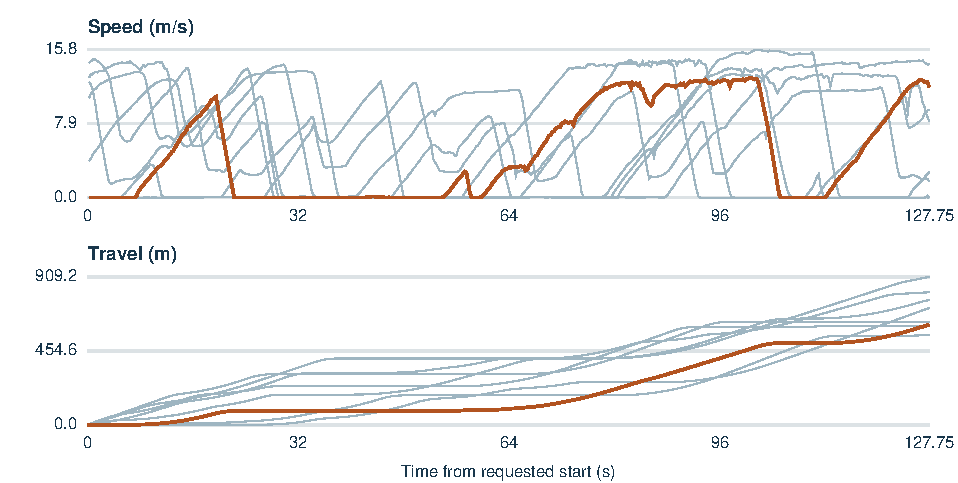
\includegraphics[width=.98\linewidth]{figures/case-bus.pdf}\end{center}
\noindent The highlighted line is the GAF-selected trace. The seven other trajectories are shown in blue-gray. Axes are scaled separately for each class.
\tab{All-candidate bus results. Units are m/s, m/s$^2$, m and percent, respectively.}{case1}{\begin{tabular}{lrrrr}\toprule
Motion & Speed $\W$ & Accel. $\W$ & Travel $\W$ & Stop \%\\\midrule
Diffusion & 0.736 & 0.078 & 95.242 & 22.3\\
Empirical & 0.985 & 0.108 & 180.760 & 31.4\\\bottomrule\end{tabular}}
\FloatBarrier

\clearpage\section{Motorcycle}
The four motorcycle references spend roughly a quarter of sampled intervals below the stop threshold. Both generators spend only about seven percent. Transporting observed profiles from the training library therefore leaves a substantial mismatch even before a learned motion distribution is used. Whether the gap reflects different route mixes or insufficient training coverage requires independent conditions.

The fixed request contains eight candidates. The random, image and coordinate rules returned candidate indices 119, 116 and 115, respectively. The observed class stop fraction across the 4 references is 24.6\%.

\begin{center}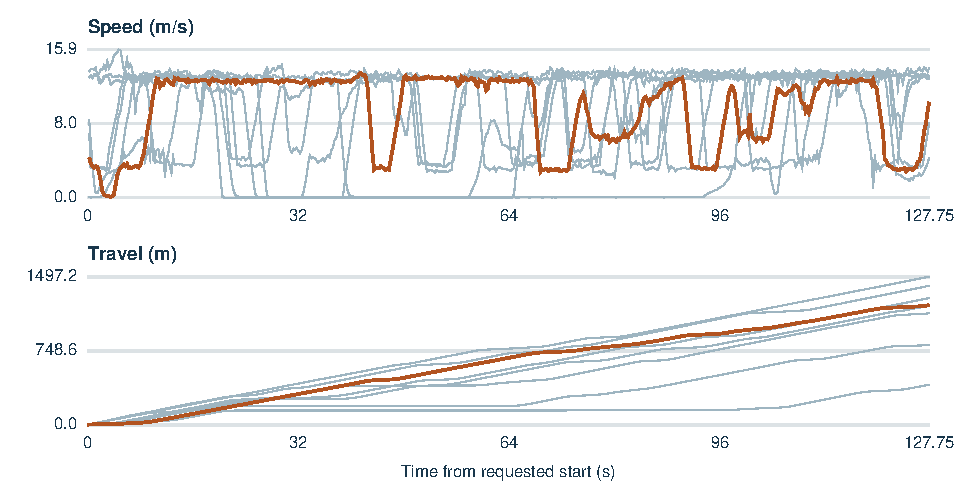
\includegraphics[width=.98\linewidth]{figures/case-motorcycle.pdf}\end{center}
\noindent The highlighted line is the GAF-selected trace. The seven other trajectories are shown in blue-gray. Axes are scaled separately for each class.
\tab{All-candidate motorcycle results. Units are m/s, m/s$^2$, m and percent, respectively.}{case2}{\begin{tabular}{lrrrr}\toprule
Motion & Speed $\W$ & Accel. $\W$ & Travel $\W$ & Stop \%\\\midrule
Diffusion & 2.068 & 0.199 & 347.655 & 7.0\\
Empirical & 2.758 & 0.265 & 367.777 & 7.4\\\bottomrule\end{tabular}}
\FloatBarrier

\clearpage\section{Private car}
Private cars account for 33 of the 53 requests. Their stop fraction is closely matched by diffusion, and their travel discrepancy is smaller than with empirical transfer. The empirical baseline, however, gives a much smaller acceleration discrepancy for this class. These results distinguish agreement on total distance from agreement on changes in speed.

The fixed request contains eight candidates. The random, image and coordinate rules returned candidate indices 133, 133 and 135, respectively. The observed class stop fraction across the 33 references is 4.8\%.

\begin{center}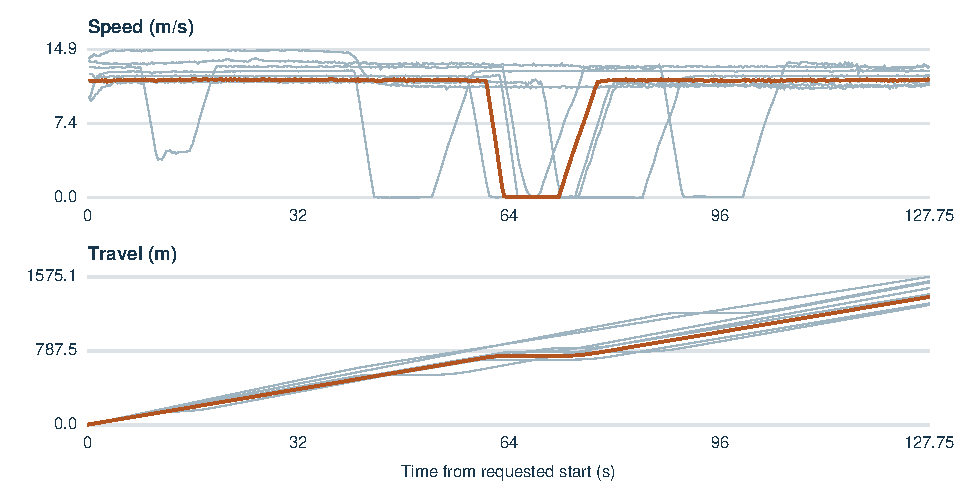
\includegraphics[width=.98\linewidth]{figures/case-private_car.pdf}\end{center}
\noindent The highlighted line is the GAF-selected trace. The seven other trajectories are shown in blue-gray. Axes are scaled separately for each class.
\tab{All-candidate private car results. Units are m/s, m/s$^2$, m and percent, respectively.}{case3}{\begin{tabular}{lrrrr}\toprule
Motion & Speed $\W$ & Accel. $\W$ & Travel $\W$ & Stop \%\\\midrule
Diffusion & 0.356 & 0.187 & 51.620 & 4.8\\
Empirical & 0.985 & 0.058 & 124.766 & 3.8\\\bottomrule\end{tabular}}
\FloatBarrier

\clearpage\section{Bicycle}
The seven observed bicycle windows spend little sampled time below the stop threshold. The two generators produce similar stop fractions of about three percent. Both acceleration discrepancies are comparatively large. Since acceleration here differentiates planar speed, quarter-second variations in the decoded geometry and timing can affect this metric even on a connected route.

The fixed request contains eight candidates. The random, image and coordinate rules returned candidate indices 62, 59 and 61, respectively. The observed class stop fraction across the 7 references is 0.1\%.

\begin{center}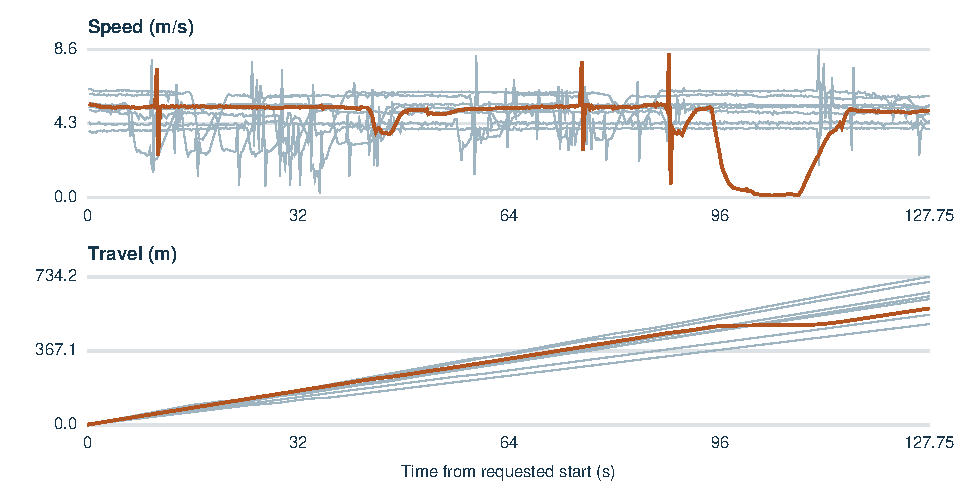
\includegraphics[width=.98\linewidth]{figures/case-bycicle.pdf}\end{center}
\noindent The highlighted line is the GAF-selected trace. The seven other trajectories are shown in blue-gray. Axes are scaled separately for each class.
\tab{All-candidate bicycle results. Units are m/s, m/s$^2$, m and percent, respectively.}{case4}{\begin{tabular}{lrrrr}\toprule
Motion & Speed $\W$ & Accel. $\W$ & Travel $\W$ & Stop \%\\\midrule
Diffusion & 0.378 & 0.651 & 55.534 & 3.0\\
Empirical & 0.505 & 0.607 & 74.275 & 3.0\\\bottomrule\end{tabular}}
\FloatBarrier

\clearpage\section{Taxi or Uber}
Only two taxi requests supply the reference distribution. In this class empirical transfer has smaller speed and travel discrepancies than diffusion, while both generators spend considerably less time nearly stationary than the two observed vehicles. The direction of the class-specific result is informative, but two vehicles provide very little information about the broader taxi population.

The fixed request contains eight candidates. The random, image and coordinate rules returned candidate indices 247, 241 and 247, respectively. The observed class stop fraction across the 2 references is 19.2\%.

\begin{center}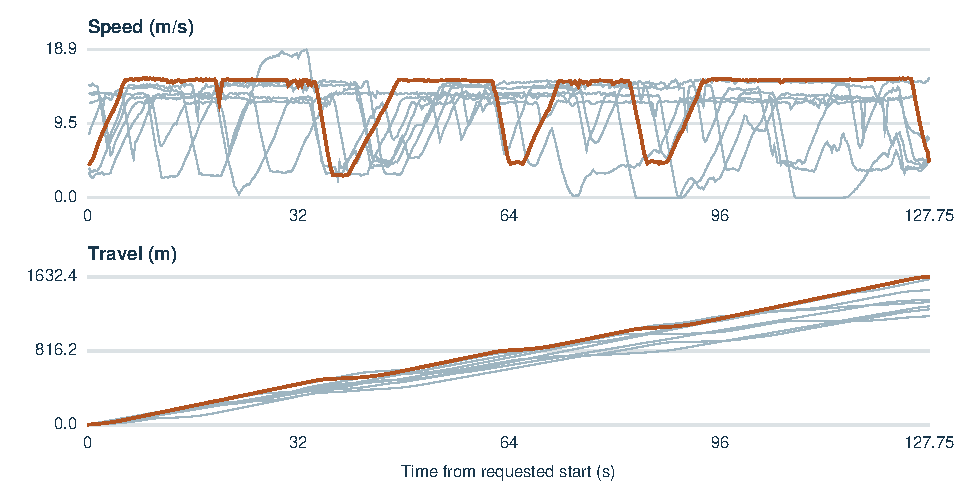
\includegraphics[width=.98\linewidth]{figures/case-taxi_or_uber.pdf}\end{center}
\noindent The highlighted line is the GAF-selected trace. The seven other trajectories are shown in blue-gray. Axes are scaled separately for each class.
\tab{All-candidate taxi or uber results. Units are m/s, m/s$^2$, m and percent, respectively.}{case5}{\begin{tabular}{lrrrr}\toprule
Motion & Speed $\W$ & Accel. $\W$ & Travel $\W$ & Stop \%\\\midrule
Diffusion & 2.681 & 0.231 & 337.019 & 2.2\\
Empirical & 2.000 & 0.155 & 258.019 & 5.3\\\bottomrule\end{tabular}}
\FloatBarrier

\endgroup

\chapter{Detailed classification and selection results}
\label{app:classification}
\section{Auditor confusion and imbalance}
The confusion summaries retain errors hidden by aggregate accuracy. Each matrix averages the row proportions of three separately trained networks on the same 182 vehicles. A cell is the share of participants of the true class predicted as the column class. Row counts are 12, 13, 31, 103, 15 and 8. An error on one taxi changes taxi recall by 12.5 points for one model.

\fig{confusion.pdf}{1}{Final auxiliary classification on observed windows. Rows are true classes and columns are predictions. Each cell averages percentages across the three frozen seeds.}{confusion}
\tab{Observed-window recognition by class. Recall and F1 are given as percentages}{auxclasses}{\begin{tabular}{lrrrrr}\toprule
Class & IDs & GAF recall & GAF F1 & TCN recall & TCN F1\\\midrule
Pedestrian & 12 & 80.6 & 85.3 & 100.0 & 98.7\\
Bus & 13 & 76.9 & 77.1 & 82.1 & 69.1\\
Motorcycle & 31 & 40.9 & 36.2 & 59.1 & 58.1\\
Private car & 103 & 75.4 & 78.0 & 82.2 & 83.8\\
Bicycle & 15 & 46.7 & 43.6 & 100.0 & 100.0\\
Taxi or Uber & 8 & 0.0 & 0.0 & 29.2 & 27.8\\\bottomrule\end{tabular}}

These matrices use observed-window recognition. The audit percentages on generated traces use requested classes on the five-class subset and two audit seeds per family. Accuracy across observed windows, six-class macro-F1 and class-macro agreement on generated candidates measure different outcomes.

\section{The complete selection comparison}
\tab{Locked five-class macro results by motion model and selection rule. Units are m/s, m/s$^2$, m and percent.}{fullselection}{\begin{tabular}{llrrrrr}\toprule
Motion & Rule & Speed & Accel. & Travel & GAF & TCN\\\midrule
Diffusion & All candidates & 1.24 & 0.27 & 177.41 & 47.48 & 77.68\\
 & Random & 1.40 & 0.28 & 206.00 & 51.85 & 89.86\\
 & GAF & 1.41 & 0.29 & 191.52 & 70.45 & 78.10\\
 & TCN & 1.44 & 0.29 & 209.30 & 47.32 & 93.18\\
 & Shuffled GAF & 1.50 & 0.28 & 195.80 & 39.55 & 76.95\\
Empirical & All candidates & 1.45 & 0.24 & 201.12 & 40.47 & 71.07\\
 & Random & 1.69 & 0.26 & 233.89 & 45.61 & 78.17\\
 & GAF & 1.89 & 0.28 & 252.55 & 63.11 & 68.41\\
 & TCN & 2.28 & 0.31 & 282.14 & 42.72 & 91.36\\
 & Shuffled GAF & 1.49 & 0.27 & 195.02 & 35.41 & 63.04\\\bottomrule\end{tabular}}

The complete-candidate row describes the distribution available to each selector. The single-selection rows serve one trace per request and therefore also use fewer samples. A difference between the full-pool and random rows alone is not an effect of feedback. The direct comparator for GAF ranking is random ranking within the same saved pool.

\section{Paired downstream contrasts}
\tab{GAF-selected augmentation minus each comparator in macro-F1 percentage points, with 95\% paired intervals}{contrasts}{\begin{tabular}{lrr}\toprule
Comparator & TCN & GRU\\\midrule
Observed only & -5.23 [-9.01, -1.65] & -1.70 [-6.42, +3.13]\\
Repeat & -1.09 [-4.02, +1.93] & +2.98 [+0.28, +5.95]\\
Time warp & -1.63 [-4.42, +1.33] & -0.46 [-2.77, +2.16]\\
Random synthetic & +1.40 [-1.54, +5.16] & +1.86 [-1.70, +5.47]\\
GAF synthetic & +0.00 [+0.00, +0.00] & +0.00 [+0.00, +0.00]\\
TCN synthetic & -0.39 [-4.41, +4.26] & +1.48 [-1.72, +4.82]\\\bottomrule\end{tabular}}

The comparison with repeated data concerns a change in motion while maintaining parent counts and class inventory. The comparison with randomly selected synthetic data isolates the value of choosing an image-preferred candidate. The comparison with observed-only training measures the practical effect of the delivered augmentation package as a whole.

\section{Per-class downstream outcomes}
\tab{Downstream per-class recall on the observed test set, in percent. Entries average the three learner initializations.}{recall}{\begin{tabular}{llrrrrrr}\toprule
Model & Group & Ped. & Bus & Moto. & Car & Bike & Taxi\\\midrule
TCN & Observed only & 100.0 & 84.6 & 51.6 & 82.5 & 100.0 & 62.5\\
 & Repeat & 88.9 & 89.7 & 48.4 & 82.8 & 100.0 & 45.8\\
 & Time warp & 91.7 & 89.7 & 48.4 & 83.5 & 100.0 & 45.8\\
 & Random synthetic & 86.1 & 92.3 & 48.4 & 82.2 & 100.0 & 33.3\\
 & GAF synthetic & 100.0 & 92.3 & 43.0 & 80.3 & 100.0 & 45.8\\
 & TCN synthetic & 83.3 & 89.7 & 51.6 & 82.8 & 100.0 & 37.5\\
GRU & Observed only & 100.0 & 41.0 & 37.6 & 81.9 & 95.6 & 66.7\\
 & Repeat & 88.9 & 46.2 & 30.1 & 81.2 & 93.3 & 58.3\\
 & Time warp & 88.9 & 53.8 & 33.3 & 80.9 & 97.8 & 62.5\\
 & Random synthetic & 86.1 & 51.3 & 31.2 & 81.9 & 95.6 & 58.3\\
 & GAF synthetic & 100.0 & 59.0 & 30.1 & 78.6 & 95.6 & 62.5\\
 & TCN synthetic & 86.1 & 53.8 & 35.5 & 79.9 & 97.8 & 54.2\\\bottomrule\end{tabular}}

The downstream task keeps pedestrians in evaluation although augmentation adds no pedestrian traces. Their recall can therefore change: adding examples of other classes changes the learned decision boundary. Improved recall in a class can also come at the expense of precision if the learner predicts the class more often. Consequently the primary six-class evaluation uses macro-F1, with per-class recall as a diagnostic.

\section{Sensitivity of the evidence}
The network could be retrained, the planner and motion sampler could draw new candidate pools, and a different set of participants could be observed. Only the last component enters the paired intervals, conditional on the existing models and routes. Resampling test participants cannot estimate sensitivity to another city or simulator version.

The whole-profile copying control has a specific interpretation. Time alignment is fixed, all 511 increments enter equally and error is measured in metres per increment. A copied short maneuver within an otherwise novel trajectory could escape detection. Two naturally similar motion sequences could also agree under a looser threshold. The empirical positive control and held-out reference comparison make the operational threshold interpretable in this study.

\clearpage
\phantomsection
\begin{thebibliography}{99}
\bibitem{salvadori} E. Salvadori, \emph{Unraveling Urban Mobility: Gramian Angular Fields for Trajectory Classification}. Master's thesis, Politecnico di Torino, 2024. \href{https://webthesis.biblio.polito.it/30378/}{PoliTo WebThesis 30378}.
\bibitem{ferreira} G. O. Ferreira, F. Dabbene, F. Malandrino and C. Ravazzi. Unraveling Urban Mobility: A Domain Knowledge-Free Trajectory Classification Using Gramian Angular Fields. \emph{IEEE Transactions on Intelligent Transportation Systems}, 27, 531--543, 2026. \href{https://doi.org/10.1109/TITS.2025.3631275}{doi:10.1109/TITS.2025.3631275}.
\bibitem{most} L. Codec\'a and J. H\"arri. Monaco SUMO Traffic (MoST) Scenario: A 3D Mobility Scenario for Cooperative ITS. \emph{SUMO User Conference}, 2018. \href{https://github.com/lcodeca/MoSTScenario}{Scenario repository}.
\bibitem{ddpm} J. Ho, A. Jain and P. Abbeel. Denoising Diffusion Probabilistic Models. \emph{Advances in Neural Information Processing Systems}, 33, 2020. \href{https://arxiv.org/abs/2006.11239}{arXiv:2006.11239}.
\bibitem{ddim} J. Song, C. Meng and S. Ermon. Denoising Diffusion Implicit Models. \emph{International Conference on Learning Representations}, 2021. \href{https://arxiv.org/abs/2010.02502}{arXiv:2010.02502}.
\bibitem{difftraj} Y. Zhu, Y. Ye, S. Zhang, X. Zhao and J. Yu. DiffTraj: Generating GPS Trajectory with Diffusion Probabilistic Model. \emph{Advances in Neural Information Processing Systems}, 36, 2023. \href{https://proceedings.neurips.cc/paper_files/paper/2023/hash/cd9b4a28fb9eebe0430c3312a4898a41-Abstract.html}{Conference proceedings}.
\bibitem{diffrn} T. Wei, Y. Lin, S. Guo, Y. Lin, Y. Huang, C. Xiang, Y. Bai and H. Wan. Diff-RNTraj: A Structure-aware Diffusion Model for Road Network-constrained Trajectory Generation. 2024. \href{https://arxiv.org/abs/2402.07369}{arXiv:2402.07369}.
\bibitem{rntrajgen} Z. Lv, Z. Fan, Z. Zhang and X. Song. Two-Stage Fine-Grained Trajectory Generation Constrained by Road Networks. \emph{IJCAI}, 2915--2923, 2026. \href{https://doi.org/10.24963/ijcai.2026/324}{doi:10.24963/ijcai.2026/324}.
\bibitem{scenario} E. Pronovost, M. R. Ganesina, N. Hendy, Z. Wang, A. Morales, K. Wang and N. Roy. Scenario Diffusion: Controllable Driving Scenario Generation With Diffusion. \emph{Advances in Neural Information Processing Systems}, 36, 2023. \href{https://arxiv.org/abs/2311.02738}{arXiv:2311.02738}.
\bibitem{wang} Z. Wang and T. Oates. Encoding Time Series as Images for Visual Inspection and Classification Using Tiled Convolutional Neural Networks. \emph{AAAI workshop}, 2015. \href{https://cdn.aaai.org/ocs/ws/ws0115/10179-46015-1-PB.pdf}{Workshop paper}.
\bibitem{resnet} K. He, X. Zhang, S. Ren and J. Sun. Deep Residual Learning for Image Recognition. \emph{IEEE Conference on Computer Vision and Pattern Recognition}, 2016. \href{https://openaccess.thecvf.com/content_cvpr_2016/html/He_Deep_Residual_Learning_CVPR_2016_paper.html}{CVPR proceedings}.
\bibitem{original} Historical trajectory project. \emph{Deep Learning Based Generative Models for Traffic Trajectory Synthesis}, revision \texttt{4773ad65}. \href{https://github.com/LiuJingting0201/Deep-Learning-Based-Generative-Models-for-Traffic-Trajectory-Synthesis/tree/4773ad65bce88d38b8b108ef5e4773fd99883c94}{Encoding source}.
\bibitem{project} Thesis experiment repository. \emph{CNR Road/GAF Trajectory Diffusion}, results snapshot \texttt{6031e3f}. \href{https://github.com/LiuJingting0201/cnr-road-gaf-diffusion/tree/6031e3f}{Private repository and frozen evaluation report}.
\end{thebibliography}

\end{document}
